\documentclass[12pt,a4paper]{report}

\usepackage{styles/dolgozat}

\usepackage{listings}
\usepackage{styles/python}

\usepackage{hyperref}

\usepackage{caption}
\usepackage{subcaption}
\usepackage{float}
\usepackage{siunitx}
\usepackage{booktabs}

\usepackage{fancyhdr}

\fancypagestyle{plain}{
  \fancyhf{}
  \fancyfoot[R]{\thepage}
}

\sisetup{
  group-separator = {\,},
  group-minimum-digits = 4,
  detect-all
}

\begin{document}

\pagestyle{empty}

{\small
Miskolci Egyetem

Gépészmérnöki és Informatikai Kar

Általános Informatikai Intézeti Tanszék
}

{\large
\begin{center}
\vglue 1.5truecm
\includegraphics[scale=0.15]{images/me_logo.png}\\
\end{center}}

\vglue 1.5truecm

{\huge
\begin{center}
\textbf{Videójátékok adatainak elemzése Python alapú gépi tanulási eszközök segítségével}
\end{center}}

\vspace*{1cm}

\begin{center}
\LARGE \textbf{Diplomamunka}
\end{center}

\vspace*{2.5truecm}

{\large
\hspace{6.5cm} \textbf{Készítette}:

%\vskip 2mm

\hspace{6.5cm} \textbf{Név}: Drig Dávid

%\vskip 1mm

\hspace{6.5cm} \textbf{Neptunkód}: \texttt{EZ3YRC}

%\vskip 1mm

\hspace{6.5cm} \textbf{Szak}: Mérnökinformatikus MSc

%\vskip 1mm

\hspace{6.5cm} Alkalmazás fejlesztő szakirány
}

\newpage


\newpage

\pagestyle{empty}

\include{cover/feladatkiiras}

\cleardoublepage
\pagenumbering{roman}
\pagestyle{plain}
\tableofcontents
\cleardoublepage
\pagenumbering{arabic}

\newpage

\pagestyle{fancy}

\Chapter{Bevezetés}

A videójátékok területén keletkező adatok elemzése napjainkban egyre fontosabb szerepet tölt be mind a kutatás, mind az ipari alkalmazások szempontjából. A Steam \cite{steam} platformon elérhető videójátékok jellemzőire, játékmenetére és teljesítményére vonatkozó adatok megfelelő feldolgozása lehetőséget teremt különböző mintázatok felismerésére, valamint prediktív és osztályozási problémák megoldására. A nagy mennyiségű és heterogén adatok kezelése azonban megfelelő adat-előkészítési és elemzési módszereket igényel.

A diplomamunka során három, a Kaggle \cite{kaggle} platformon elérhető, Steamhez kapcsolódó videojáték-adathalmaz kerül feldolgozásra. Az adatkészletek kezdetben különálló munkafüzetekben kerülnek elemzésre, az egyes adathalmazok szerkezetének és minőségének megismerése érdekében. Az előzetes vizsgálatot követően az adatok tisztítása és normalizálása történik meg annak érdekében, hogy az eltérő forrásból származó adatok egységes formában legyenek kezelhetők.

A normalizált adathalmazok ezt követően összevonásra kerülnek egy egységes, nagyobb adatkészletté. Az adatbázis logikus felépítése és a hatékony elemzés érdekében az összevont adathalmaz további, tematikusan elkülönülő táblákra kerül bontásra, biztosítva az adatok átlátható kezelését.

Az előkészített adatokon statisztikai és feltáró vizsgálatok kerülnek elvégzésre az adatok közötti összefüggések feltárása érdekében. Ezt követően a dolgozat a gépi tanulás területére fókuszál, különös tekintettel az osztályozási problémák megoldására. A Python \cite{python} programozási nyelv és annak gépi tanulást támogató könyvtárai segítségével különböző osztályozó algoritmusok kerülnek alkalmazásra és összehasonlításra.

A dolgozat célja annak bemutatása, hogy a megfelelő adat-előkészítés és -feldolgozás milyen mértékben befolyásolja a gépi tanulási modellek teljesítményét, valamint hogy az alkalmazott osztályozási módszerek mennyire hatékonyan alkalmazhatók videojáték-adatok elemzésében.

\Chapter{Adatok előkészítése}

Ebben a fejezetben a dolgozat során felhasznált adatok forrása és előkészítési folyamata kerül bemutatásra. A fejezet első része rövid áttekintést ad a Steam \cite{steam} szolgáltatásról, valamint az onnan származó, a Kaggle \cite{kaggle} platformon elérhető adathalmazok jellemzőiről, beleértve azok formátumát és mennyiségi tulajdonságait. Ezt követően a vizsgált adathalmazok részletesebb áttekintése történik meg, különös tekintettel az egyes adatkészletek külön notebookokban végzett elemzésére és az adatelőkészítés során szerzett gyakorlati tapasztalatokra.

\Section{Steam szolgáltatás és a kezelt adatai}

A következő alfejezetek röviden bemutatják a Steam \cite{steam} szolgáltatást mint
adatforrást, valamint a dolgozat során felhasznált adatok eredetét,
elérhetőségét és alapvető jellemzőit. Emellett áttekintésre kerülnek az
adatelőkészítés és elemzés során alkalmazott fejlesztőkörnyezetek és
szoftveres eszközök is.

\subsection{A Steam szolgáltatás áttekintése}

A Steam \cite{steam} egy digitális videojáték-disztribúciós platform, amelyet a Valve Corporation \cite{valve} üzemeltet, és amely világszerte az egyik legnagyobb online videojáték-áruháznak számít. A szolgáltatás lehetőséget biztosít videojátékok vásárlására, letöltésére és frissítésére, valamint különböző közösségi funkciók – például értékelések, fórumok és statisztikák – elérésére.

A Steam platformon elérhető videojátékokhoz számos, nyilvánosan hozzáférhető adat kapcsolódik. Ezek közé tartoznak többek között a játékok alapvető jellemzői (például cím, megjelenési dátum, fejlesztő, kiadó), műfaji besorolásuk, felhasználói értékelések, valamint egyes esetekben teljesítményre és népszerűségre vonatkozó mutatók. Az ilyen típusú adatok különösen alkalmasak statisztikai elemzésre és gépi tanulási módszerek alkalmazására.

A Steam által kezelt adatok mennyisége és sokfélesége miatt a platform gyakran szolgál adatforrásként kutatási és elemzési célokra. A játékokhoz kapcsolódó strukturált adatok lehetőséget biztosítanak különböző mintázatok feltárására, például a műfajok közötti különbségek, a felhasználói értékelések alakulása vagy a játékok népszerűségének vizsgálata során. Ennek köszönhetően a Steamhez kapcsolódó adathalmazok jól illeszkednek adatfeldolgozási és gépi tanulási feladatok bemutatásához. A Steam digitális videojáték-disztribúciós platform logóját a \ref{fig:steam_logo} ábra szemlélteti.

\begin{figure}[H]
    \centering
    \includegraphics[width=0.3\textwidth]{images/Steam_icon_logo.pdf}
    \caption{A Steam digitális videojáték-disztribúciós platform logója}\cite{steam_logo}
    \label{fig:steam_logo}
\end{figure}

\subsection{A Kaggle platform szerepe}

A Kaggle \cite{kaggle} egy online adatmegosztó és adatverseny-platform, amely elsősorban adatkutatási és gépi tanulási feladatokhoz biztosít nyilvánosan elérhető adathalmazokat. A platformon a felhasználók különböző forrásokból származó, dokumentált adatállományokat oszthatnak meg, amelyek kutatási és oktatási célokra egyaránt felhasználhatók.

A dolgozat során alkalmazott adathalmazok a Kaggle platformon kerültek publikálásra, és Steamhez kapcsolódó, nyilvános adatok feldolgozott formáit tartalmazzák. A Kaggle egységes hozzáférést, verziókezelést és leírást biztosít az adatkészletekhez, ami megkönnyíti azok összehasonlítható és reprodukálható feldolgozását. A Kaggle adatmegosztó és adatkutatási platform vizuális
azonosítóját a \ref{fig:kaggle_logo} ábra mutatja be.

\begin{figure}[H]
    \centering
    \includegraphics[width=0.25\textwidth]{images/Kaggle_logo.pdf}
    \caption{A Kaggle adatmegosztó és adatkutatási platform logója}\cite{kaggle_logo}
    \label{fig:kaggle_logo}
\end{figure}

\subsection{Az elemzés során használt eszközök}

Az adatok feldolgozása és elemzése Python \cite{python} programozási nyelv
felhasználásával történt. A fejlesztéshez a Visual Studio Code \cite{vscode}
fejlesztőkörnyezet, valamint Jupyter Notebook \cite{jupyter} alapú munkafüzetek
kerültek alkalmazásra, amelyek lehetővé tették az interaktív
adatelemzést és az egyes lépések dokumentálását.

Az adatok kezeléséhez és előfeldolgozásához elsősorban a \texttt{pandas} \cite{pandas}
és \texttt{NumPy} \cite{numpy} könyvtárak kerültek felhasználásra, míg a
vizualizációk elkészítéséhez a \texttt{matplotlib} \cite{matplotlib} és
\texttt{seaborn} \cite{seaborn} csomagok szolgáltak alapul. A gépi tanulási és
regressziós számítások során a \texttt{scikit-learn} \cite{scikit} könyvtár
egyes komponensei kerültek alkalmazásra.

\subsection{Letöltés, formátum és mennyiségi jellemzők}

A dolgozat során felhasznált adatok a Kaggle \cite{kaggle} platformon elérhető,
Steamhez \cite{steam} kapcsolódó nyilvános adathalmazokból származnak.
Az adatkészletek manuális letöltéssel kerültek beszerzésre a Kaggle webes felületén
keresztül, amelyhez felhasználói fiók megléte szükséges.
A letöltött állományok tömörített formában voltak elérhetők, és kicsomagolást
követően különálló adatfájlokat (CSV és JSON formátumú táblákat) tartalmaztak.

Az elsőként vizsgált adatkészlet a
\textit{Steam Store Games (Clean dataset)} \cite{a},
amely a továbbiakban \textit{A adathalmazként} kerül hivatkozásra.
Az adathalmaz a Steam áruházban elérhető videojátékok különböző jellemzőit
tartalmazza, többek között műfaji besorolásokat, leírásokat, címkéket és
becsült tulajdonosi adatokat.
Az adatok a Steam Store és a SteamSpy \cite{steamspy} API-k felhasználásával
kerültek összegyűjtésre, és elsősorban a 2019 májusáig megjelent játékokra
vonatkoznak.
Az A adathalmaz több, egymással logikailag összefüggő CSV fájlból áll,
amelyek külön relációként értelmezhetők; ezek rekord- és attribútumszáma
táblánként eltérő.

A második adathalmaz a Kaggle platformon
\textit{Steam Games Dataset} \cite{b} néven elérhető,
amely a továbbiakban \textit{B adathalmazként} kerül megjelölésre.
Az adathalmaz egyetlen, nagyméretű CSV/JSON alapú táblát tartalmaz,
amely a Steam API és a SteamSpy szolgáltatás adatain alapul.
A feltáró adatelemzés során a CSV formátum került alkalmazásra.
A B adathalmaz összesen \num{111452} rekordot és 40 attribútumot tartalmaz.

A harmadik vizsgált adatkészlet a
\textit{Steam Games Dataset 2025} \cite{c},
amely a továbbiakban \textit{C adathalmazként} kerül hivatkozásra.
Az adathalmaz a Steam áruház weboldalának automatizált feldolgozásával,
valamint a Steam API és a SteamSpy adatainak felhasználásával készült,
és 2025 márciusáig bezárólag tartalmaz adatokat.
Az adatok több CSV fájlban érhetők el, beleértve nyers és előfeldolgozott
változatokat is, amelyek táblánként eltérő attribútumkészlettel rendelkeznek.

Az adatkészletek eltérő szerkezete, fájlformátuma és attribútumkészlete
indokolttá tette az adatok előzetes tisztítását, normalizálását,
valamint egy egységesített adatszerkezet kialakítását,
amely a későbbi elemzési és gépi tanulási feladatok alapját képezi.
A felhasznált adathalmazok főbb mennyiségi jellemzőit,
táblánkénti bontásban, a \ref{tab:datasets} táblázat foglalja össze.

\begin{table}[H]
\centering
\begin{tabular}{|l|l|c|c|}
\hline
\textbf{Adathalmaz} & \textbf{Tábla} & \textbf{Rekordok száma} & \textbf{Attribútumok száma} \\
\hline
A & steam.csv & \num{27075} & 18 \\
A & steam\_description\_data.csv & \num{27334} & 4 \\
A & steam\_media\_data.csv & \num{27332} & 5 \\
A & steam\_requirements\_data.csv & \num{27319} & 6 \\
A & steamspy\_tag\_data.csv & \num{29022} & 372 \\
\hline
B & games.csv & \num{111452} & 40 \\
\hline
C & games\_march2025\_cleaned.csv & \num{89618} & 47 \\
C & games\_march2025\_full.csv & \num{94948} & 47 \\
C & games\_may2024\_cleaned.csv & \num{83646} & 46 \\
C & games\_may2024\_full.csv & \num{87806} & 46 \\
\hline
\end{tabular}
\caption{A felhasznált adathalmazok táblánkénti mennyiségi jellemzői}
\label{tab:datasets}
\end{table}

\section{A vizsgálandó adathalmaz áttekintése}

A vizsgált adathalmazok előzetes feltárása és elemzése különálló
Jupyter \cite{jupyter} munkafüzetekben történt, adathalmazonként
elkülönítve. Az A \cite{a}, B \cite{b} és C \cite{c} adathalmazok
önálló munkafüzetekben kerültek feldolgozásra, ami lehetővé tette az
egyes adatkészletek szerkezetének, tartalmának és sajátosságainak
részletes megismerését, valamint az adatokra jellemző problémák korai
azonosítását. Az egyes vizsgálatok részletes dokumentációja a dolgozathoz
mellékelt \textit{notebooks} jegyzékében érhető el.

A külön munkafüzetek alkalmazása elősegítette a feldolgozási folyamat
átláthatóságát, mivel az egyes adathalmazok eltérő szerkezettel,
formátummal és attribútumkészlettel rendelkeztek. Ez a megközelítés
lehetővé tette, hogy az adattisztítási, feltáró elemzési és
előfeldolgozási lépések az adott adathalmaz sajátosságaihoz igazodjanak,
anélkül hogy azok összekeveredtek volna más adatforrások feldolgozásával.

Az egyes adathalmazok esetében azonos alapvető vizsgálati lépések kerültek
elvégzésre. Ezek célja az adatok általános állapotának felmérése, valamint
a későbbi feldolgozási lépések megalapozása volt. A munkafüzetekben az
alábbi vizsgálatok történtek meg:
\begin{itemize}
    \item az adatok betöltése és szerkezetének áttekintése, beleértve az
    oszlopok számát, adattípusokat és a hiányzó értékek előfordulását,
    \item alapvető statisztikai leíró mutatók vizsgálata,
    \item a főbb attribútumok vizualizációja, például eloszlások,
    időbeli trendek és kategória-gyakoriságok megjelenítése,
    \item adatminőségi problémák, kiugró értékek és jellegzetes mintázatok
    azonosítása.
\end{itemize}

Az előzetes feltáró elemzés során néhány, az adathalmazok jellegét jól
szemléltető vizualizáció is készült. Ezek célja nem a részletes
statisztikai elemzés, hanem az adatok alapvető szerkezetének,
eloszlásainak és időbeli mintázatainak bemutatása.

Az \textit{A adathalmaz} esetében a játékok átlagos árának időbeli
alakulását vizsgáltam. A \ref{fig:mean} ábra az éves átlagárak változását
mutatja, amely alapján hosszabb távú trendek és árszintváltozások
azonosíthatók. Az ábra rávilágít arra, hogy az átlagár nem állandó,
hanem az egyes időszakokban számottevő ingadozást mutat, ami a
Steam-platform üzleti modelljének és a megjelenő játékok összetételének
változásával hozható összefüggésbe.

\begin{figure}[H]
    \centering
    \includegraphics[width=1.0\textwidth]{images/mean.png}
    \caption{Az A adathalmazban szereplő játékok átlagos ára évenként}
    \label{fig:mean}
\end{figure}

Szintén az \textit{A adathalmazhoz} kapcsolódóan a műfaji eloszlás
vizsgálata is megtörtént. A \ref{fig:top20} ábra a Top~20 műfaj
előfordulási gyakoriságát szemlélteti. Jól látható, hogy néhány műfaj
jelentős dominanciával rendelkezik, míg a ritkább kategóriák csak
korlátozott számban jelennek meg. Ez a jelenség fontos szempont az
adathalmaz későbbi elemzésekor, mivel a műfajok közötti egyenlőtlen
eloszlás torzíthat bizonyos statisztikai következtetéseket.

\begin{figure}[H]
    \centering
    \includegraphics[width=1.0\textwidth]{images/top20.png}
    \caption{Az A adathalmaz Top~20 műfajának előfordulási gyakorisága}
    \label{fig:top20}
\end{figure}

A \textit{B adathalmaz} esetében a játékok által támogatott platformok
szerinti megoszlás került vizsgálatra. A \ref{fig:platforms} ábra
bemutatja, hogy a Windows platform támogatása messze domináns, míg a
macOS és Linux rendszerek lényegesen kisebb arányban jelennek meg. Ez az
eltérés jól szemlélteti a platformfüggetlenség korlátait, valamint
magyarázatot adhat bizonyos platform-specifikus hiányosságokra az
adatokban.

\begin{figure}[H]
    \centering
    \includegraphics[width=1.0\textwidth]{images/platforms.png}
    \caption{A B adathalmazban szereplő játékok száma támogatott platformonként}
    \label{fig:platforms}
\end{figure}

A \textit{C adathalmaz} elemzése során a játékok Metacritic értékeinek
időbeli alakulása került előtérbe. A \ref{fig:metacritic} ábra a
Metacritic pontszámok és a kiadási év kapcsolatát ábrázolja. Az ábra
alapján megfigyelhető, hogy az értékelések jelentős szórást mutatnak
minden időszakban, ugyanakkor az idő előrehaladtával a pontszámok
eloszlása kiegyensúlyozottabbá válik. Ez arra utal, hogy a modern
időszakban a megjelenő játékok minősége stabilabb, illetve az
értékelési mechanizmus egységesebbé vált.

\begin{figure}[H]
    \centering
    \includegraphics[width=1.0\textwidth]{images/metacritic.png}
    \caption{A C adathalmazban szereplő játékok Metacritic értékei a kiadási év függvényében}
    \label{fig:metacritic}
\end{figure}

A feltáró vizsgálatok során szerzett tapasztalatok rávilágítottak arra,
hogy az adathalmazok közötti különbségek — például az eltérő
attribútumnevek, hiányzó értékek és formátumbeli eltérések — jelentős
hatással vannak a későbbi összevonási és normalizálási lépésekre. A
kezdeti, elkülönített feldolgozás ezért kulcsszerepet játszott egy
egységes, közös adatszerkezet kialakításának előkészítésében. Az itt
bemutatott előzetes elemzések eredményei szolgáltak alapul a következő
fejezetben részletezett adattisztítási, normalizálási és
adathalmaz-összevonási folyamatokhoz.

\Chapter{Adatok egységes struktúrába szervezése}

Ebben a fejezetben a vizsgált adathalmazok egységes adatstruktúrába szervezésének folyamata kerül bemutatásra. A fejezet célja annak ismertetése, hogy a korábban elkülönítve feldolgozott, eltérő szerkezetű adatkészletek hogyan alakíthatók át egy közös, jól strukturált adatsémává, amely alkalmas további elemzési és gépi tanulási feladatok elvégzésére.

A fejezet első részében az adathalmazok közötti kapcsolatok és relációs sémák elemzése történik meg, amely alapot szolgáltat az adatok logikus felépítéséhez. Ezt követően bemutatásra kerülnek az alkalmazott normalizálási lépések, valamint azok indoklása az adatbázis-tervezési alapelvek figyelembevételével. A továbbiakban az adatok tisztításával kapcsolatos feladatok kerülnek ismertetésre, különös tekintettel a hiányzó és inkonzisztens értékek kezelésére. A fejezet zárásaként az egyes adathalmazok összevonásának (merge) folyamata kerül bemutatásra, amelynek eredményeként egy egységes, elemzésre kész adatstruktúra jön létre.

\Section{Relációs sémák elemzése}

Az adathalmazok egységes struktúrába szervezésének első lépéseként az egyes adatkészletek relációs sémáinak elemzése történt meg. A vizsgálat célja az volt, hogy feltárja az adatok belső szerkezetét, az attribútumok közötti kapcsolatokat, valamint azokat az azonosítókat, amelyek az adathalmazok későbbi összekapcsolását lehetővé teszik.

A feldolgozás során az A, B és C adathalmazokhoz külön relációs sémák kerültek kialakításra. Ezek a sémák az egyes adatkészletek logikai felépítését írják le, kiemelve a fő entitásokat, azok attribútumait, valamint az elsődleges és idegen kulcsokat. Az elkülönített sémák vizsgálata lehetővé tette az adathalmazok közötti hasonlóságok és szerkezeti eltérések azonosítását.

Az A adathalmaz relációs sémája a videojátékok alapvető jellemzőit tartalmazza, és referenciapontként szolgált a további adatkészletek integrálása során. A B és C adathalmazok sémái kiegészítő információkat hordoznak, amelyek eltérő attribútumkészlettel rendelkeznek, ugyanakkor közös játékazonosítók mentén kapcsolhatók az A adathalmazhoz.

Az A, B és C adathalmazok sémáinak elemzését követően került kialakításra a D adathalmaz relációs sémája, amely az eredeti adatkészletek összevonásával létrehozott, egységes adatstruktúrát írja le. A D adathalmaz sémája már a normalizálási és tisztítási lépések eredményét tükrözi, és közvetlen alapját képezi a további elemzési és gépi tanulási feladatoknak.

A sémák elemzése során meghatározásra került az adathalmazok összevonásának prioritási sorrendje is. Az integrálás során a C adathalmaz szolgált elsődleges adatforrásként, mivel ez tartalmazta a legfrissebb információkat. A B, majd az A adathalmaz adatai kiegészítő jelleggel kerültek figyelembevételre, elsősorban azon attribútumok esetében, amelyek a C adathalmazban nem, vagy csak hiányosan álltak rendelkezésre. Ez a prioritási sorrend biztosította, hogy az összevont adathalmaz a lehető legaktuálisabb adatokat tükrözze.

A relációs sémák vizsgálata rávilágított arra, hogy az eltérő szerkezetű adathalmazok integrálása csak előzetes normalizálási és adatelőkészítési lépések után valósítható meg hatékonyan. A feltárt kapcsolatok és függőségek szolgáltak alapul a következő alfejezetben bemutatott normalizálási folyamatokhoz, valamint az adathalmazok összevonásának megvalósításához.

\Section{Normalizálás}

A normalizálás célja az adatredundancia csökkentése, az adatintegritás biztosítása, valamint az adatok logikus, karbantartható és bővíthető szerkezetbe rendezése. A dolgozat során alkalmazott normalizálási lépések az első, második és harmadik normálforma (1NF–3NF) követelményeit követik, figyelembe véve az egyes adathalmazok eltérő szerkezeti sajátosságait.

\subsection{Az A adathalmaz normalizálása}

\subsubsection{Első normálforma (1NF)}

Az eredeti CSV állomány több olyan attribútumot tartalmazott, amelyek nem atomi értékeket vettek fel. Ilyenek voltak például a több elemet tartalmazó címkék, műfajok, kategóriák, platformok, valamint a képernyőképeket és videókat leíró mezők. Az első normálforma követelménye szerint minden attribútumnak oszthatatlan, atomi értéket kell tartalmaznia, ezért ezek az összetett és listaértékű attribútumok külön táblákba kerültek.

A listaértékű adatok kezelésére külön entitások és kapcsolótáblák kerültek kialakításra. A címkék, műfajok, platformok és kategóriák önálló táblákban kerültek tárolásra, míg a játékok és ezen attribútumok közötti több–több kapcsolatokat kapcsolótáblák reprezentálják. Az A adathalmazban a címkék eredetileg több különálló oszlopban szerepeltek, amelyek a feldolgozás során egységes szerkezetbe kerültek összevonásra, és egy szótárjellegű (dictionary) struktúrában lettek eltárolva a további normalizálási lépések megkönnyítése érdekében. 

A médiatartalmak – képernyőképek és videók – esetében minden egyes elem külön rekordként került eltárolásra. A képernyőképeket tartalmazó attribútumok további bontása is szükségessé vált, mivel az eredeti adathalmaz teljes méretű és előnézeti képeket egyetlen struktúrában tárolt. Ennek megfelelően a képernyőképek külön attribútumokra kerültek bontásra a teljes felbontású (\textit{screenshots\_full}) és az előnézeti (\textit{screenshots\_thumbs}) képek elkülönített kezelésére. Hasonló módon a videók esetében külön attribútumok kerültek kialakításra az eltérő típusú és felbontású médiaforrások kezelésére (\textit{movies\_thumbnail}, \textit{movies\_max}, \textit{movies\_480}). A rendszerkövetelmények szintén felbontásra kerültek operációs rendszer és követelménytípus (minimum, ajánlott) szerint. 

A rendszerkövetelmények esetében az eredeti, platformonként elkülönített mezők egységes struktúrába kerültek átszervezésre, ahol az operációs rendszer (\textit{windows}, \textit{mac}, \textit{linux}) külön attribútumban jelenik meg. A követelmények típusa egy külön \textit{type} mező segítségével került megkülönböztetésre, amely minimum és ajánlott értékeket vehet fel, míg a konkrét hardver- és szoftverkonfiguráció a \textit{requirements} mezőben kerül tárolásra.


\subsubsection{Második normálforma (2NF)}

A második normálforma biztosítása érdekében vizsgálatra kerültek az elsődleges kulcstól való részleges függőségek. Az A adathalmaz központi táblája a \textit{game} entitás, amelynek elsődleges kulcsa az \textit{appid}. Azokat az attribútumokat, amelyek ugyan az \textit{appid}-tól függenek, de nem a játék alapadatait írják le, külön táblákba kerültek szétválasztásra.

Ennek eredményeként önálló táblák jöttek létre a részletes és rövid leírások kezelésére, a támogatási információk (például URL és e-mail cím) tárolására, valamint a médiához kapcsolódó elemek elkülönítésére. A rendszerkövetelmények kezelése szintén külön táblában történt, az operációs rendszer és a követelménytípus figyelembevételével.

\subsubsection{Harmadik normálforma (3NF)}

A harmadik normálforma megvalósítása során a tranzitív függőségek megszüntetésére került sor. A fejlesztők és kiadók adatai önálló entitásokba kerültek, és a játékokhoz kapcsolótáblákon keresztül kapcsolódnak. Ez a megoldás lehetővé tette a redundáns szöveges adatok elkerülését és az adatok konzisztens kezelését. Az adathalmazban szereplő fejlesztőkre és kiadókra vonatkozó attribútumok elnevezései az eredeti struktúrát követték (\textit{developer}, \textit{publisher}), azonban a normalizált sémában ezek önálló entitásokként jelennek meg, biztosítva az egységes elnevezést és a redundanciamentes adatkezelést.

Hasonló módon a kategóriák, műfajok, címkék és platformok esetében is külön táblák tárolják az egyedi értékeket, míg a játékokkal való kapcsolatukat kizárólag azonosítók segítségével megvalósított kapcsolótáblák reprezentálják. A több–több kapcsolatok minden esetben explicit módon, kapcsolótáblák segítségével kerültek kezelésre.

\subsubsection{Összegzés}

A normalizálási folyamat eredményeként az A adathalmaz relációs sémája több, logikailag elkülönülő entitásból épül fel. A központi \textit{game} tábla mellett önálló táblák jöttek létre a leírások, támogatási információk, médiatartalmak, rendszerkövetelmények, valamint a különböző kategorizáló attribútumok kezelésére. A sémában minden több–több kapcsolat külön kapcsolótáblán keresztül valósul meg, biztosítva az adatok redundanciamentes tárolását.

Az A adathalmaz normalizálási lépései biztosították az adatredundancia minimalizálását, a tranzitív függőségek megszüntetését, valamint a listaértékű és összetett attribútumok önálló táblákba történő szétválasztását. A kialakított relációs séma jól strukturált, karbantartható és alkalmas arra, hogy alapjául szolgáljon a további adatintegrációs és gépi tanulási feladatoknak.

Az A adathalmaz részletes attribútumleírását és az egyes mezők jelentését tartalmazó adatleíró (data dictionary) a dolgozat mellékletei között érhető el. Az A adathalmaz normalizálatlan relációs sémáját a \ref{fig:A_unnormalized} ábra, míg a normalizált relációs sémát a
\ref{fig:A_normalized} ábra szemlélteti.


\begin{figure}[H]
    \centering
    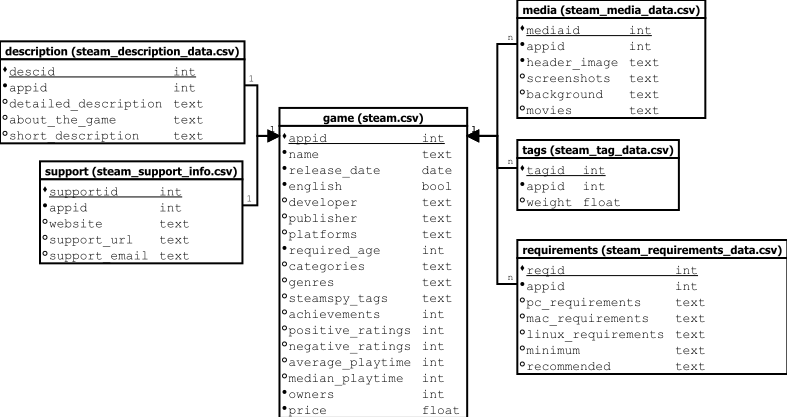
\includegraphics[width=1.0\textwidth]{images/A_unnormalized.pdf}
    \caption{Az A adathalmaz normalizálatlan relációs sémája}
    \label{fig:A_unnormalized}
\end{figure}

\begin{figure}[H]
    \centering
    \includegraphics[width=1.0\textwidth]{images/A_normalized.pdf}
    \caption{Az A adathalmaz normalizált relációs sémája}
    \label{fig:A_normalized}
\end{figure}

\subsection{A B adathalmaz normalizálása}

\subsubsection{Első normálforma (1NF)}

Az eredeti \textit{games.csv} állomány több ismétlődő és listaértékű attribútumot tartalmazott, például képernyőképeket, címkéket, kategóriákat, műfajokat, támogatott nyelveket, szinkronhangokat és játékcsomagokat. Az első normálforma követelményeinek megfelelően ezek az attribútumok felbontásra kerültek, és az adatok atomi értékeket tartalmazó táblákba lettek átszervezve.

A médiatartalmak – képek és videók – külön táblákban kerültek tárolásra, ahol minden elem önálló rekordot képez. A kategóriák, műfajok és címkék esetében önálló entitások jöttek létre, míg a játékokkal való több–több kapcsolatukat kapcsolótáblák reprezentálják. A nyelvek külön táblában kerültek eltárolásra, és a játékokhoz való kapcsolódásuk felirat és szinkronhang szerinti bontásban történt. A platformok kezelése szintén normalizált formában, külön táblák és kapcsolatok segítségével valósult meg.

A játékcsomagok összetett szerkezete miatt többszintű modell került kialakításra, amely elkülöníti a csomag alapadatait és azok alelemeit, biztosítva az adatok áttekinthető és atomi szintű tárolását.

\subsubsection{Második normálforma (2NF)}

A második normálforma biztosítása érdekében a részleges függőségek megszüntetésére került sor. A központi \textit{game} tábla elsődleges kulcsa az \textit{appid}, amelyhez kizárólag a játék alapadatai tartoznak. Azok az attribútumok, amelyek nem közvetlenül a játék leírását szolgálják, külön relációkba kerültek.

Ennek eredményeként önálló táblák jöttek létre a támogatási információk, médiatartalmak, kategorizáló attribútumok, nyelvek, fejlesztők, kiadók, platformok és csomagadatok kezelésére. A több–több kapcsolatok minden esetben asszociatív táblák segítségével kerültek megvalósításra, biztosítva az adatok egyértelmű és redundanciamentes összekapcsolását.

\subsubsection{Harmadik normálforma (3NF)}

A harmadik normálforma megvalósítása során a tranzitív függőségek megszüntetése volt a cél. A címkék, műfajok, nyelvek, fejlesztők, kiadók, kategóriák, platformok és csomagok megnevezései önálló táblákban kerültek eltárolásra, így elkerülhetővé vált a redundáns szöveges adatok ismétlődése.

A nyelvek kezelése egységes módon történt, ahol az egyes nyelvek egyszer kerülnek tárolásra, és külön kapcsolótáblák jelzik, hogy egy adott játék rendelkezik-e feliratokkal vagy hanggal az adott nyelven. Ez a megoldás megszüntette a korábbi listaértékű mezők közötti redundanciát. A játékcsomagok többszintű felépítése szintén a tranzitív függőségek elkerülését és az adatok logikus strukturálását szolgálta.

\subsubsection{Összegzés}

A normalizálás eredményeként a B adathalmaz relációs sémája egy jól strukturált, több entitásból álló adatmodellt alkot. A központi \textit{game} tábla mellett önálló relációk kezelik a támogatási információkat, médiatartalmakat, kategorizáló attribútumokat, nyelveket, fejlesztőket, kiadókat, platformokat, valamint a játékcsomagok és azok al-elemeinek adatait. A séma minden több–több kapcsolatot külön kapcsolótáblákon keresztül valósít meg.

A B adathalmaz normalizálási folyamata eredményeként egy tiszta, jól strukturált adatmodell jött létre, amely megfelel az első három normálforma követelményeinek. A kialakított séma atomi értékeket tartalmaz, megszünteti a részleges és tranzitív függőségeket, valamint külön táblákban kezeli az összetett és listaértékű mezőket. Az alkalmazott struktúra jól bővíthető, karbantartható, és minimális adatredundanciát biztosít a további feldolgozási és elemzési lépésekhez.

A B adathalmaz normalizált sémájához tartozó adatleíró (data dictionary), amely az attribútumok jelentését és típusát részletezi, a dolgozat mellékleteiben található. A B adathalmaz normalizálatlan relációs sémáját a \ref{fig:B_unnormalized} ábra, míg a normalizált relációs sémát a \ref{fig:B_normalized} ábra szemlélteti.

\begin{figure}[H]
    \centering
    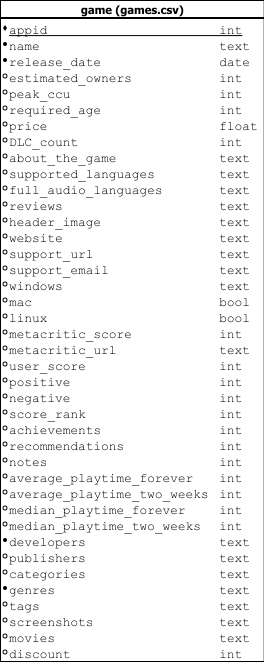
\includegraphics[width=0.6\textwidth]{images/B_unnormalized.pdf}
    \caption{A B adathalmaz normalizálatlan relációs sémája}
    \label{fig:B_unnormalized}
\end{figure}

\begin{figure}[H]
    \centering
    \includegraphics[width=1.0\textwidth]{images/B_normalized.pdf}
    \caption{A B adathalmaz normalizált relációs sémája}
    \label{fig:B_normalized}
\end{figure}

\subsection{A C adathalmaz normalizálása}

A C adathalmaz normalizálásának kiindulópontját négy, időben és feldolgozottságban eltérő CSV-fájl képezte: a 2024 májusi és a 2025 márciusi adatállományok nyers (\textit{full}) és előfeldolgozott (\textit{cleaned}) változatai. A \textit{full} állományok a Steam \cite{steam} áruházból származó teljes, nyers adatokat tartalmazták, míg a \textit{cleaned} változatok már előzetes tisztításon átesett, duplikációktól mentes adatokat biztosítottak.

A 2025-ös adatkészletek a korábbi verziókhoz képest egy további attribútummal is bővültek, amely a játékok aktuális kedvezményét (\textit{discount}) írja le. A normalizálás során az eltérő időpontokból és szerkezetből adódó különbségek egységes kezelése kiemelt szempont volt.

\subsubsection{Első normálforma (1NF)}

Az eredeti CSV-fájlok több olyan attribútumot tartalmaztak, amelyek nem atomi értékeket vettek fel. Ilyenek voltak például a képernyőképek, címkék, kategóriák, műfajok, valamint a támogatott feliratokat és szinkronhangokat tartalmazó mezők. Az első normálforma követelményeinek megfelelően ezek az összetett és listaértékű attribútumok külön relációkba kerültek.

A normalizálás során önálló entitások jöttek létre többek között a médiatartalmak, képernyőképek, videók, leírások, kategóriák, műfajok, nyelvek, platformok és játékcsomagok kezelésére. A nyelvi attribútumok két külön relációban kerültek eltárolásra, megkülönböztetve a feliratokat és a szinkronhangokat. Ez a felosztás lehetővé tette a nyelvi támogatás pontosabb és redundanciamentes kezelését.

\subsubsection{Második normálforma (2NF)}

A második normálforma biztosítása érdekében a részleges függőségek megszüntetésére került sor. A játékokat leíró központi tábla elsődleges kulcsa az \textit{appid}, amelyhez kizárólag a játék alapadatai tartoznak. Azok az attribútumok, amelyek ugyan az \textit{appid}-tól függnek, de nem közvetlenül a játék alapjellemzőit írják le, külön relációkba kerültek.

Önálló táblák jöttek létre többek között a támogatási információk, médiatartalmak, leírások, kategóriák, műfajok, nyelvek, fejlesztők, kiadók, címkék, platformok és játékcsomagok kezelésére. A redundáns szöveges ismétlődések megszüntetésre kerültek azáltal, hogy az egyes entitások megnevezései saját táblákban szerepelnek, míg a játékokkal való kapcsolatukat kizárólag azonosítók biztosítják.

\subsubsection{Harmadik normálforma (3NF)}

A harmadik normálforma megvalósítása során a tranzitív függőségek megszüntetése volt a cél. A kategóriák, műfajok, nyelvek, fejlesztők, kiadók, címkék, platformok és csomagok megnevezései önálló entitásokban kerültek eltárolásra, míg a játékokkal való kapcsolatukat külön asszociatív táblák írják le.

A játékcsomagok kezelése háromszintű struktúrában valósult meg. A játék és a csomag közötti kapcsolatot egy kapcsolótábla reprezentálja, míg a csomagok alapadatai és azok alelemei külön relációkban kerültek eltárolásra. Ez a megoldás biztosítja az összetett csomagstruktúrák áttekinthető és redundanciamentes kezelését.

\subsubsection{Összegzés}

A normalizálás eredményeként a C adathalmaz relációs sémája egy egységes, jól strukturált adatmodellt alkot. A központi \textit{game} tábla mellett önálló relációk kezelik a támogatási információkat, médiatartalmakat, leírásokat, kategorizáló attribútumokat, nyelveket, fejlesztőket, kiadókat, platformokat, valamint a játékcsomagok és azok al-elemeinek adatait. A 2025-ös adatkészletekben megjelenő \textit{discount} attribútum a végső sémában is elkülönítve, konzisztens módon került kezelésre.

A C adathalmaz normalizálása során négy különálló, eltérő időpontból származó CSV-fájl került egységes relációs struktúrába szervezésre. Az alkalmazott normalizálási lépések biztosítják az első három normálforma követelményeinek teljesülését, elkülönítik a felirat- és hangnyelveket, valamint strukturált módon kezelik a játékcsomagokat. A kialakított séma csökkenti az adatredundanciát, elősegíti az adatok konzisztenciáját, és rugalmasan kezeli a 2024-es és 2025-ös adatforrások közötti eltéréseket, így megfelelő alapot biztosít a további integrációs és elemzési feladatokhoz.

A C adathalmaz normalizált sémájához tartozó adatleíró (data dictionary), amely az egyes attribútumok jelentését és típusát részletezi, a dolgozat mellékleteiben található. A C adathalmaz normalizálatlan relációs sémáját a\ref{fig:C_unnormalized} ábra, míg a normalizált relációs sémát a \ref{fig:C_normalized} ábra szemlélteti.

\begin{figure}[H]
    \centering
    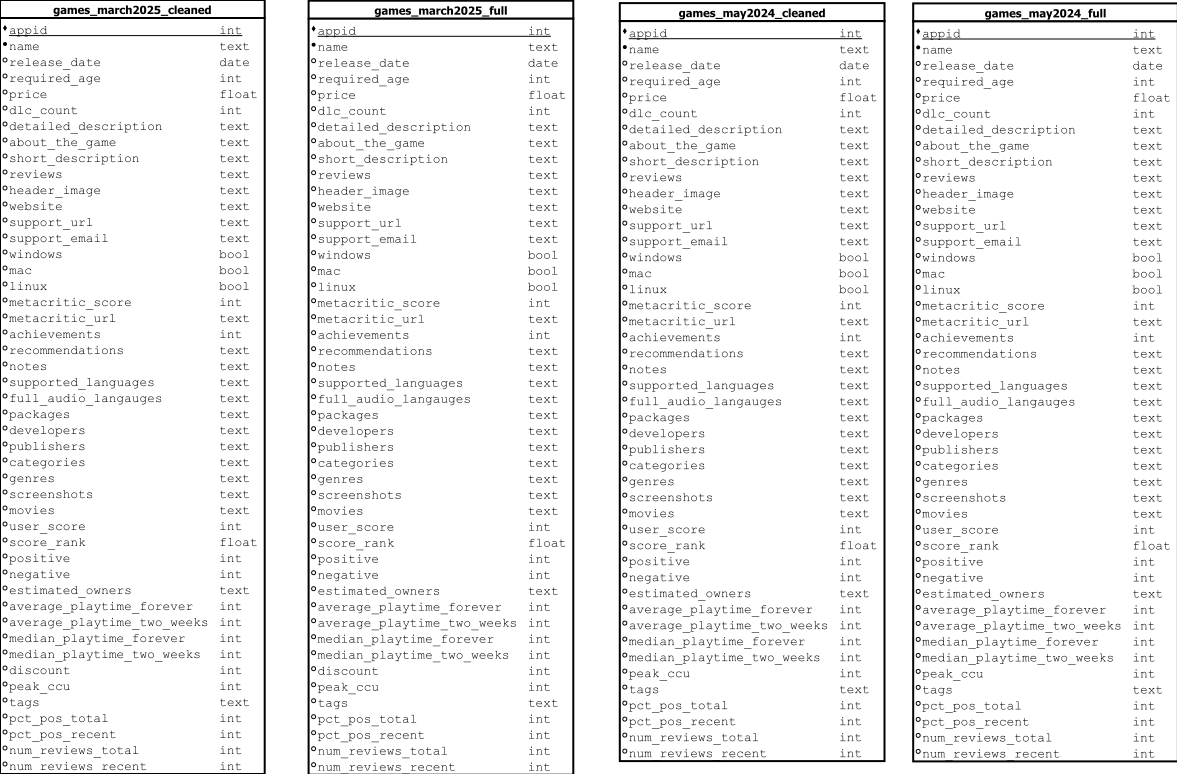
\includegraphics[width=1.0\textwidth]{images/C_unnormalized.pdf}
    \caption{A C adathalmaz normalizálatlan relációs sémája}
    \label{fig:C_unnormalized}
\end{figure}

\begin{figure}[H]
    \centering
    \includegraphics[width=1.0\textwidth]{images/C_normalized.pdf}
    \caption{A C adathalmaz normalizált relációs sémája}
    \label{fig:C_normalized}
\end{figure}

\subsection{A D adathalmaz normalizálása}

A D adathalmaz egységes relációs sémája az A, B és C adathalmazok összevonásával és strukturális egységesítésével jött létre. Kiindulási alapként több, eltérő forrásból származó CSV-fájl szolgált, amelyek részben különböző szerkezettel, eltérő attribútumkészlettel és eltérő időpontokból származó adatokat tartalmaztak. A normalizálás célja egy olyan konzisztens, redundanciamentes adatmodell kialakítása volt, amely egységesen kezeli az eltérő forrásokból származó információkat.

A 2024-es és 2025-ös adatkészletek közötti egyik lényeges eltérés, hogy a 2025-ös verziók egy további attribútumot is tartalmaztak, amely a játékok aktuális kedvezményét (\textit{discount}) írja le. Az egységesítés során ezek a forrásbeli különbségek kezelhető módon kerültek beépítésre a végső sémába.

\subsubsection{Első normálforma (1NF)}

Az összevont CSV-fájlok több olyan attribútumot tartalmaztak, amelyek nem atomi értékeket vettek fel, például címkéket, műfajokat, kategóriákat, támogatott nyelveket, hangnyelveket, csomagstruktúrákat és rendszerkövetelményeket JSON formátumban. Az első normálforma követelményeinek megfelelően ezek az összetett és listaértékű mezők önálló relációkba kerültek.

Az ilyen attribútumok kezelésére külön entitások és kapcsolótáblák jöttek létre, amelyek a játékokkal való kapcsolatot asszociatív módon írják le. Ide tartoznak többek között a felirat és szinkronhangok kezelése, a címkék, műfajok, kategóriák, platformok, valamint a többszintű csomagszerkezetek és a rendszerkövetelmények strukturált tárolása. Ez a felbontás biztosítja, hogy minden attribútum atomi értéket vegyen fel, és megfeleljen az első normálforma előírásainak.

\subsubsection{Második normálforma (2NF)}

A második normálforma megvalósítása érdekében a részleges függőségek megszüntetésére került sor. A D adathalmaz központi táblája a \textit{game} entitás, amelynek elsődleges kulcsa az \textit{appid}. Azok az attribútumok, amelyek az \textit{appid}-tól függnek, de nem a játék alapadatait írják le, külön relációkba kerültek.

Ennek eredményeként önálló táblák jöttek létre többek között a leírások, támogatási információk, médiatartalmak, képernyőképek, videók, rendszerkövetelmények, nyelvek, tulajdonosi tartományok, valamint a csomagok és azok alelemeinek kezelésére. Ez a szétválasztás biztosítja, hogy minden nem kulcsattribútum teljes mértékben függjön az elsődleges kulcstól.

\subsubsection{Harmadik normálforma (3NF)}

A harmadik normálforma teljesítése érdekében a tranzitív függőségek megszüntetésre kerültek. Az ismétlődő szöveges attribútumok – például címkék, műfajok, kategóriák, nyelvek, platformok, fejlesztők és kiadók – önálló entitásokban kerültek eltárolásra, míg a játékokkal való kapcsolatukat külön asszociatív táblák reprezentálják.

A több-több kapcsolatok minden esetben kapcsolótáblák segítségével kerülnek kezelésre, biztosítva az adatok konzisztenciáját és a redundancia minimalizálását. A játékcsomagok kezelése háromszintű struktúrában valósult meg, amely elkülöníti a játék–csomag kapcsolatot, a csomag alapadatait és a csomagok alelemeit. Ez a megoldás lehetővé teszi az összetett csomagszerkezetek áttekinthető és bővíthető kezelését.

\subsubsection{Összegzés}

A D adathalmaz relációs sémája az A, B és C adathalmazok összevonásával létrehozott, egységes adatmodellt képvisel. A kialakított struktúra biztosítja az első három normálforma követelményeinek teljesülését, megszünteti a redundáns és nem atomi mezőket, valamint strukturált módon kezeli a több-több kapcsolatokat és az összetett csomagstruktúrákat. A séma képes kezelni az eltérő adatforrások közötti különbségeket, bővíthető a jövőbeni adatokkal, és stabil alapot biztosít a további elemzési és gépi tanulási feladatokhoz.

A D adathalmaz normalizált sémájához tartozó adatleíró (data dictionary), amely az egyes attribútumok jelentését és típusát részletezi, a dolgozat mellékleteiben található.

A D adathalmaz normalizált relációs sémájának SQL-alapú megvalósítása a dolgozat mellékleteiben található. Az ott bemutatott SQL definíciók a végső adatmodellt írják le, és egyértelműen jelölik, hogy az egyes táblák és attribútumok mely forrásadathalmazokból (A, B vagy C) származnak. A D adathalmaz egységesített, normalizált relációs sémája a \ref{fig:D_schema} ábrán látható.

\begin{figure}[H]
    \centering
    \includegraphics[width=0.95\textwidth]{images/D_schema.pdf}
    \caption{A D adathalmaz egységes, normalizált relációs sémája}
    \label{fig:D_schema}
\end{figure}

\Section{Adathalmazok összefésülése}

Ebben az alfejezetben az A, B és C adathalmazok összefésülésének folyamata kerül bemutatásra. Az adathalmazok egyesítése során az eltérő forrásokból származó adatok strukturális különbségeinek kezelése, az attribútumok egységesítése, valamint az adatok konzisztenciájának biztosítása volt a fő cél. Az összefésülési folyamat eredményeként jött létre a végső, egységes D adathalmaz, amely a további elemzések alapját képezi.

Az alfejezet bemutatja az adathalmazok összefésülésének logikai lépéseit, a folyamat vizuális áttekintését, valamint a megvalósításhoz használt módszereket. Emellett kitér a merge során végrehajtott ellenőrzésekre és azokra a döntésekre, amelyek biztosították az adatok helyes és következetes integrációját.

\subsection{Az összefésülés logikai folyamata}

Az adathalmazok összefésülésének folyamata az A, B és C forrásadatok strukturált és kontrollált egyesítését mutatja be. A folyamat célja egy egységes, konzisztens adatmodell létrehozása volt, amely a különböző forrásokból származó információkat egységes szerkezetben tartalmazza. Az összefésülés lépéseit és azok egymásra épülését a \ref{fig:merge_process} ábra szemlélteti.

\begin{figure}[H]
    \centering
    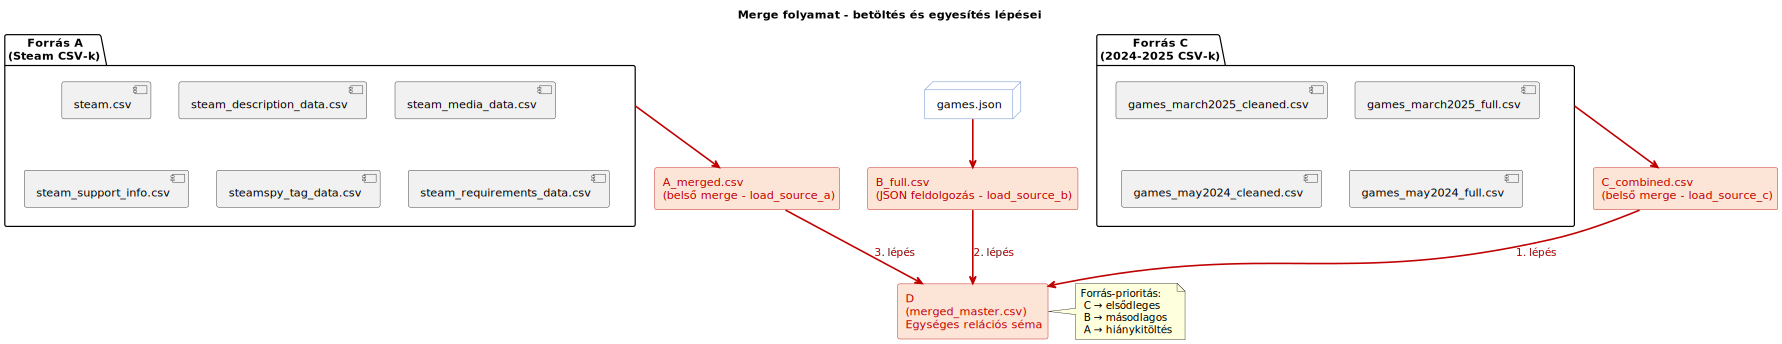
\includegraphics[width=1.0\textwidth]{images/merge_folyamat.pdf}
    \caption{Az A, B és C adathalmazok összefésülésének folyamata}
    \label{fig:merge_process}
\end{figure}


Az ábra PlantUML \cite{plantuml} alapú forráskódja külön fájlban is elérhető (\textit{merge\_process.puml}), amely a folyamat reprodukálhatóságát és dokumentáltságát biztosítja.

\subsubsection{Az összefésülés lépései}

Az \ref{fig:merge_process} ábrán bemutatott folyamat három fő részlépésből áll, amelyek során az egyes forrásadathalmazok önállóan kerülnek feldolgozásra és előkészítésre az egységesítés előtt.

Első lépésként a C forrás feldolgozása történik meg, amely során a 2024-es és 2025-ös CSV-fájlok kerülnek összevonásra és előtisztításra. Ennek eredményeként jön létre a \textit{C\_combined.csv} állomány, amely már egységes szerkezetben tartalmazza az időben eltérő adatforrások adatait.

Második lépésként a B forrás feldolgozása következik, ahol a JSON formátumban elérhető SteamSpy \cite{steamspy} adatok normalizálása és táblásítása történik meg. A feldolgozás eredményeként a \textit{B\_full.csv} állomány jön létre, amely strukturált formában tartalmazza a másodlagos adatforrásból származó információkat.

Harmadik lépésként az A forrás feldolgozása valósul meg, amely során a több CSV-fájlból álló Steam-metaadatok \cite{steam} belső összevonása történik meg. Az eredmény az \textit{A\_merged.csv} állomány, amely az A adathalmaz egységesített változatát tartalmazza.

\subsubsection{Források egyesítése és prioritási sorrend}

Az előfeldolgozott részadathalmazok ezt követően egyesítésre kerülnek egy közös adatállományba. Az összefésülés során meghatározott prioritási sorrend biztosítja, hogy az eltérő források közötti átfedések esetén a legaktuálisabb és legmegbízhatóbb adatok kerüljenek felhasználásra.

A prioritási sorrend az alábbiak szerint alakult:
\begin{itemize}
    \item a C adathalmaz elsődleges forrásként szolgált,
    \item a B adathalmaz másodlagos forrásként került bevonásra,
    \item az A adathalmaz kiegészítő, kitöltő szerepet töltött be.
\end{itemize}

A folyamat eredményeként egy egységes relációs struktúra jött létre (\textit{merged\_master.csv}), amely már közvetlenül alkalmas volt a normalizálási lépések végrehajtására és az SQL-alapú adatbázis felépítésére.

\subsection{Az összefésülés megvalósítása}

Ebben az alfejezetben az A, B és C adathalmazok összefésülésének szoftveres megvalósítása kerül bemutatásra. A merge-folyamat egy moduláris felépítésű Python \cite{python} projektként valósult meg, amely külön kezeli a forrásadatok betöltését, az előfeldolgozási és tisztítási lépéseket, valamint az adatok egységesítését és ellenőrzését. A bemutatott kódrészletek nem a teljes implementációt fedik le, hanem a összefésülés-folyamat szempontjából lényeges, nem triviális megoldásokat szemléltetik.

\subsubsection{A merge-kód felépítése}

Az adathalmazok összefésülésében az alábbi főbb modulok vesznek részt:

\begin{itemize}
    \item \texttt{merge/sources} – az A, B és C forrásadatok beolvasásáért és előtisztításáért felelős modulok,
    \item \texttt{merge/utils} – általános segédfüggvények az adatkezelési, tisztítási, normalizálási és merge-lépések támogatására,
    \item \texttt{merge/visualization} – a mergelt adathalmazra épülő statisztikai ábrák és összefoglaló vizualizációk generálása,
    \item \texttt{merge/output} – a futtatás során keletkező kimeneti állományok és ábrák gyűjtőmappája.
\end{itemize}

A teljes merge-folyamatot a \texttt{merge/main.ipynb} Jupyter \cite{jupyter} munkafüzet vezérli, míg a globális beállításokat és paramétereket a \texttt{merge/config.py} konfigurációs állomány tartalmazza.

\subsubsection{Kiemelt kódrészletek}

A teljes kódbázis részletes ismertetése nem szükséges, ezért az alábbiakban csak néhány olyan megoldás kerül bemutatásra, amelyek jól szemléltetik az összefésülés során alkalmazott logikai döntéseket és adatkezelési stratégiákat. A projekt minden modulja és függvénye részletes dokumentációval (docstringekkel) van ellátva.

\paragraph{Hiányzó adatok kitöltése forrásprioritás alapján}

A merge egyik kulcseleme egy olyan függvény (\ref{lst:missing}), amely a céladatkészlet hiányzó mezőit más forrásokból pótolja. A kitöltés az \textit{appid} alapján történik, és kizárólag azokat az oszlopokat érinti, amelyek mindkét adathalmazban megtalálhatók. A megoldás biztosítja, hogy a források közötti prioritás (C → B → A) ütközésmentesen érvényesüljön.

\begin{python}[caption={Hiányzó adatok pótlása},captionpos=b,label={lst:missing}]
def fill_missing_from_source(d: pd.DataFrame,
                             src: pd.DataFrame) -> pd.DataFrame:
    src = src.copy()
    src["appid"] = src["appid"].astype(str)

    common_cols = [col for col in src.columns if col in d.columns]

    merged = d.merge(
        src[common_cols],
        on="appid",
        how="left",
        suffixes=("", "_src")
    )

    for col in common_cols:
        if col != "appid":
            merged[col] = merged[col].combine_first(merged[f"{col}_src"])
            merged.drop(columns=[f"{col}_src"], inplace=True)

    return merged
\end{python}

\paragraph{Listaértékű attribútumok egyesítése}

A címkék, műfajok, kategóriák és platformok esetében gyakori volt, hogy ugyanazon játékhoz több forrásból is listaértékű adatok tartoztak. Ezek összevonására egy deduplikáló segédfüggvény (\ref{lst:dedup}) került alkalmazásra, amely a különböző forrásokból származó listákat egyesíti, miközben az ismétlődő elemeket eltávolítja.

\begin{python}[caption={Deduplikáló segédfüggvény},captionpos=b,label={lst:dedup}]
def dedup_join(*lists):
    combined = []
    for lst in lists:
        if isinstance(lst, list):
            combined.extend(lst)
    return list(dict.fromkeys(combined))
\end{python}

\paragraph{Képernyőképek több forrásból történő kombinálása}

A képernyőképek kezelése során az A, B és C adathalmazokból származó adatok egyesítése index-alapú leképezéssel történt. A megoldás lehetővé tette, hogy a különböző forrásokból származó képernyőképek a prioritási sorrendnek megfelelően kerüljenek összefűzésre, miközben az egységes attribútumstruktúra megmaradt.

\paragraph{Nyelvi mezők többlépcsős tisztítása}

A nyelvi mezők feldolgozása az egyik legösszetettebb lépés volt, mivel az A, B és C forrásokban eltérő, gyakran zajos formátumban jelentek meg. A normalizálás két egymásra épülő tisztítási lépésből állt: az első lépés a nyers adatok egységesítését és alapvető tisztítását végezte el, míg a második lépés a nyelvnevek szabványosítását és a kontextusfüggő hibák kiszűrését valósította meg. A folyamat eredményeként egy konzisztens, relációs adatbázisba illeszthető nyelvlista jött létre.

\paragraph{A B forrás JSON állományainak feldolgozása}

A B adathalmaz JSON formátumú, beágyazott szerkezete miatt külön betöltési és feldolgozási logika készült. A feldolgozás során az egyes játékokhoz tartozó mezők strukturált rekordokká alakultak, a listaértékű attribútumok normalizált formában kerültek eltárolásra, majd az adatok egységes Pandas DataFrame struktúrába rendeződtek. A feldolgozás fő lépéseit a \ref{lst:b} kódrészlet mutatja be.

\begin{python}[caption={B adathalmaz feldolgozása},captionpos=b,label={lst:b}]
def load_source_b(base_path: str) -> pd.DataFrame:
    file_path = os.path.join(base_path, "games.json")
    with open(file_path, "r", encoding="utf-8") as f:
        dataset = json.load(f)

    records = []
    for appID, game in dataset.items():
        fields = ["name", "release_date", "estimated_owners", "price"]
        record = {key: game.get(key) for key in fields}
        record["appid"] = str(appID)

        list_fields = ["packages", "developers", "publishers", "genres"]
        record.update({f: game.get(f, []) for f in list_fields})

        tags = game.get("tags", {})
        record["tags"] = tags if isinstance(tags, dict) else {}

        records.append(record)

    df_b = pd.DataFrame(records)
    df_b["release_date"] = pd.to_datetime(df_b["release_date"], 
    errors="coerce")
\end{python}

\subsubsection{Logolás és ellenőrzés a merge folyamat során}

Az összefésülési folyamat teljes egészében részletes naplózással került végrehajtásra. A logolás lehetővé tette a forrásfájlok betöltésének, a feldolgozott rekordok számának, valamint az egyes tisztítási és összefésülési lépések nyomon követését. A naplóállományok segítségével a teljes feldolgozási folyamat visszakövethetővé vált, és az esetleges hibák vagy inkonzisztenciák gyorsan azonosíthatók voltak. 

Az összefésülési folyamat során keletkező naplóbejegyzések egy különálló logfájlba kerülnek mentésre. A részletes futási információk, figyelmeztetések és státuszüzenetek a \texttt{merge/merge\_log.txt} állományban kerülnek rögzítésre, amely lehetővé teszi a feldolgozási lépések utólagos ellenőrzését és visszakövetését.


A logolás kiterjedt többek között a forrásadatok betöltésére, az ideiglenes rész-adathalmazok mentésére, az adatok egyesítésére, valamint a végső, egységes D adathalmaz előállítására. Ez a megközelítés biztosította a merge-folyamat átláthatóságát és reprodukálhatóságát.

\Section{Az egységesített adathalmaz felbontása}

Az összefésülési folyamat eredményeként létrejött \textit{merged\_master.csv} egyetlen, nagyméretű, összevont adatállományt tartalmazott. A split folyamat célja az volt, hogy ebből az egységesített táblából tematikus, normalizált CSV-fájlok jöjjenek létre, amelyek közvetlenül megfelelnek a kialakított relációs adatmodell struktúrájának.

A feldolgozás során minden egyes résztábla létrehozása külön függvények segítségével történt. Az elkészült CSV-fájlok a \texttt{split/} könyvtárba kerültek mentésre. A kód futása közben részletes naplózás készült, amely a \texttt{split\_log.txt} állományban rögzíti a feldolgozás egyes lépéseit, biztosítva a folyamat átláthatóságát és visszakövethetőségét.

\subsection{A split folyamat lépései}

A teljes felosztási folyamatot a \texttt{main()} függvény automatizálja, amely az alábbi fő lépésekből áll:
\begin{itemize}
    \item a \textit{merged\_master.csv} állomány betöltése,
    \item az egyes relációknak megfelelő résztáblák létrehozása,
    \item a generált táblák mentése CSV formátumban,
    \item a folyamat közben a feldolgozási lépések naplózása.
\end{itemize}

\subsection{A létrehozott táblák}

A split folyamat során az alábbi CSV-fájlok kerülnek előállításra:
\begin{itemize}
    \item \textit{game.csv} – a videojátékok alapadatai,
    \item \textit{description.csv} – részletes, rövid és „about” leírások,
    \item \textit{media.csv} – fejléc- és háttérképek,
    \item \textit{screenshots.csv} – teljes méretű és előnézeti képernyőképek,
    \item \textit{movies.csv} – videók (Full HD, 480p és előnézeti változatok),
    \item \textit{support.csv} – támogatási URL-ek és e-mail címek,
    \item \textit{requirements.csv} – minimum és ajánlott rendszerkövetelmények operációs rendszer szerint,
    \item \textit{platforms.csv} és \textit{game\_platform.csv} – platformok és kapcsolótábla,
    \item \textit{genres.csv} és \textit{game\_genre.csv} – műfajok és kapcsolótábla,
    \item \textit{categories.csv} és \textit{game\_category.csv} – kategóriák és kapcsolótábla,
    \item \textit{packages.csv}, \textit{sub\_package.csv} és \textit{game\_package.csv} – Steam csomagok és kapcsolatok,
    \item \textit{developers.csv} és \textit{game\_developer.csv} – fejlesztők,
    \item \textit{publishers.csv} és \textit{game\_publisher.csv} – kiadók,
    \item \textit{tags.csv} és \textit{game\_tag.csv} – címkék és súlyozásuk,
    \item \textit{languages.csv} – normalizált nyelvlista,
    \item \textit{game\_subtitles.csv} és \textit{game\_audio\_language.csv} – felirat- és hangnyelvek.
\end{itemize}

\subsection{A split folyamat működési elvei}

A résztáblák előállítása során minden feldolgozási lépés azonos alapelveket követett. A master táblából kizárólag az adott relációhoz tartozó oszlopok kerültek kiválasztásra, a listaértékű mezők normalizálása megtörtént, és szükség esetén új azonosítók kerültek generálásra (például műfajok, címkék vagy nyelvek esetében). A több–több kapcsolatok kezelésére minden esetben külön kapcsolótáblák jöttek létre.

A split folyamat eredményeként az eredetileg egyetlen, összevont adatállományból olyan, logikailag elkülönített és normalizált táblák jöttek létre, amelyek teljes mértékben megfelelnek a relációs adatbázis-tervezési elveknek, és közvetlenül alkalmasak SQL-alapú adatbázisba történő importálásra.


\Chapter{Leíró statisztikák}

Ez a fejezet a korábbi fejezetekben előállított, egységesített \textit{merged} adathalmazra épül, amely a különböző forrásokból származó videojáték-metaadatok összefésült és normalizált nézetét tartalmazza. Az adat-előkészítési, összevonási és felbontási lépések eredményeként létrejött adatállomány lehetővé teszi a Steam \cite{steam} platformon megjelenő videojátékok jellemzőinek átfogó, statisztikai szemléletű vizsgálatát.

A fejezet célja az adatok alapvető szerkezeti és mennyiségi tulajdonságainak feltárása, valamint a legfontosabb mintázatok és tendenciák bemutatása leíró statisztikai eszközök segítségével. Az elemzések nem prediktív jellegűek, hanem az adathalmaz megértését, konzisztenciájának ellenőrzését és a későbbi gépi tanulási feladatok előkészítését szolgálják.

A fejezet első alfejezete az előzetes vizsgálatokra fókuszál, amelyek során az adatok alapvető eloszlásai, időbeli lefedettsége és főbb numerikus jellemzői kerülnek áttekintésre. Ezt követően a grafikonokra épülő alfejezet vizuális eszközök segítségével mutatja be a játékmegjelenések, értékelések és egyéb kulcsfontosságú attribútumok közötti összefüggéseket és trendeket.

\Section{Előzetes vizsgálatok}

Az előzetes vizsgálatok célja a \textit{merged} adathalmaz szerkezetének és
alapvető minőségi jellemzőinek áttekintése. Ebben a részben a források közötti
átfedések mértékét, a rekordok forrás szerinti megoszlását, valamint az összevonás
során releváns integritási problémákat ellenőrzöm, amelyek közvetlenül befolyásolják
a későbbi statisztikai elemzések és adatbázisba importálás megbízhatóságát.

\subsection{Források közötti átfedések -- Venn-diagram}

Az A, B és C forrásadatok közötti átfedések vizsgálatához Venn-diagram készült, amely az \textit{appid} azonosítók alapján szemlélteti, hogy mely rekordok érhetők el kizárólag egy adott adatforrásban, illetve melyek jelennek meg több forrás metszetében. A vizsgálat célja annak ellenőrzése volt, hogy az összevonás során mekkora a források közötti lefedettség, valamint milyen mértékű kiegészítő információ várható az egyes adathalmazoktól.

\begin{figure}[H]
    \centering
    \includegraphics[width=0.85\textwidth]{images/venn_diagram.png}
    \caption{Az A, B és C források közötti átfedések Venn-diagramja \textit{appid} alapján}
    \label{fig:venn_sources}
\end{figure}

A \ref{fig:venn_sources} ábrán látható, hogy a források közötti legnagyobb átfedés a B és C adathalmazok között figyelhető meg (\num{79888} közös \textit{appid}), míg az A adathalmaz jellemzően a B forrással fed át (\num{24433} közös \textit{appid}). Az egyedi rekordok száma a B és C források esetében alacsonyabb (\num{5731} csak B-ben, 161 csak C-ben), míg az A forrás különálló elemei (\num{1234}) és az A--C közös, de B-ben nem szereplő rekordok (\num{1400}) kisebb részarányt képviselnek. A diagram alapján megállapítható, hogy a D adathalmaz kialakítása során a B és C forrás együttes használata biztosítja a legnagyobb lefedettséget, míg az A adathalmaz elsősorban kiegészítő szerepet tölt be.

A Venn-diagram az \texttt{merge/venn\_diagram.png} állományba került mentésre, az elemszámokat tartalmazó összefoglaló táblázat pedig \texttt{venn\_table.csv} formátumban is elérhető.


\subsection{Forrásösszegzés (Source Summary)}

A merged master táblában minden rekordhoz tartozik egy \textit{sources} mező, amely jelzi, hogy az adott sor mely eredeti adatforrás(ok)ból származik (A, B, C). Ez lehet egyetlen forrás (például \textit{A}), vagy több forrás kombinációja (például \textit{B,C} vagy \textit{A,B,C}).

A forrásonkénti rekordösszesítő célja annak feltérképezése volt, hogy a végső D adathalmaz milyen arányban épül az egyes forrásokra, illetve milyen mértékű átfedés figyelhető meg közöttük. Az elemzés során meghatározásra kerül:
\begin{itemize}
    \item hány rekord származik kizárólag az A, B vagy C forrásból,
    \item hány rekord érkezik két forrás kombinációjából,
    \item valamint hány rekord található meg mindhárom adatforrásban.
\end{itemize}

Az összesítés eredménye egy CSV formátumú táblázatban kerül mentésre, amely a \texttt{source\_summary.csv} fájlban érhető el. Ez a táblázat jól áttekinthető módon mutatja meg az egyes forráskombinációkhoz tartozó rekordok számát, valamint azt is, hogy az adott kombináció tartalmazza-e az A, B vagy C forrást.

A forrásonkénti rekordösszesítés kulcsszerepet játszik annak megértésében, hogy az adathalmazok mennyire fedik egymást, és hogy az összevonás során a meghatározott prioritási sorrend (C → B → A) hogyan jelenik meg a végső adatmodellben.

Az alábbi \ref{lst:save} függvény mutatja be a forrásonkénti rekordösszesítő előállításának megvalósítását:

\begin{python}[caption={Forrásonkénti rekordösszesítő előállításának megvalósítása},captionpos=b,label={lst:save}]
def save_source_summary(d: pd.DataFrame, output_dir: str):

    summary = d["sources"].value_counts().reset_index()
    summary.columns = ["source_combination", "record_count"]

    summary["contain_A"] = summary["source_combination"].str.contains("A")
    summary["contain_B"] = summary["source_combination"].str.contains("B")
    summary["contain_C"] = summary["source_combination"].str.contains("C")

    output_file = os.path.join(output_dir, "source_summary.csv")
    summary.to_csv(output_file, index=False, encoding="utf-8-sig")

    logging.info(f"Source summary saved: {output_file}")
\end{python}

\subsection{Integritásvizsgálat}

Az integritásvizsgálat célja a merged tábla alapvető adatminőségi problémáinak feltárása, amelyek az összevonási folyamat során vagy a forrásadatok sajátosságai miatt jelenhetnek meg. Az ellenőrzések elsősorban a kulcsazonosítók, a kötelező mezők és a dátumformátumok konzisztenciájára fókuszálnak, mivel ezek hibái közvetlenül befolyásolják a későbbi normalizálási lépések és az SQL importálás biztonságát.

A vizsgálat az alábbi ellenőrzéseket hajtja végre:
\begin{itemize}
    \item duplikált \textit{appid} értékek azonosítása,
    \item hiányzó \textit{appid} értékek számlálása,
    \item hiányzó játéknevek (\textit{name}) ellenőrzése,
    \item hiányzó vagy üres forrásjelölés (\textit{sources}) vizsgálata,
    \item érvénytelen \textit{release\_date} értékek detektálása dátumkonverzióval.
\end{itemize}

Az ellenőrzés eredménye egy külön CSV jelentésben kerül mentésre \texttt{integrity\_report.csv} néven, amely a hibák számát ellenőrzésenként összesítve tartalmazza. Ez a jelentés az összefésülés-folyamat utólagos ellenőrzésére és dokumentálására is alkalmas.

Az alábbi \ref{lst:integrity} függvény szemlélteti az integritásvizsgálat megvalósítását:

\begin{python}[caption={Integritásvizsgálat megvalósítása},captionpos=b,label={lst:integrity}]
def validate_integrity(d: pd.DataFrame, output_dir: str):

    results = []

    results.append({
        "check": "Duplicate appids",
        "error_count": d["appid"].duplicated().sum()
    })

    results.append({
        "check": "Missing appids",
        "error_count": d["appid"].isna().sum()
    })

    if "name" in d.columns:
        results.append({
            "check": "Missing names",
            "error_count": d["name"].isna().sum()
        })

    if "sources" in d.columns:
        results.append({
            "check": "Missing sources",
            "error_count": (d["sources"] == "").sum()
        })

    if "release_date" in d.columns:
        invalid = pd.to_datetime(d["release_date"], 
        errors="coerce").isna().sum()
        results.append({
            "check": "Invalid release_date",
            "error_count": invalid
        })

    integrity_df = pd.DataFrame(results)

    output_file = os.path.join(output_dir, "integrity_report.csv")
    integrity_df.to_csv(output_file, index=False, encoding="utf-8-sig")

    logging.info(f"Integrity check completed, saved to {output_file}")
\end{python}


\Section{Grafikonok}

A fejezet következő része a legfontosabb leíró statisztikai eredményeket
vizuális formában mutatja be. A grafikonok célja, hogy szemléletesen kiemeljék
a megjelenések időbeli alakulását, a források szerinti különbségeket, valamint
a műfaji és szezonális mintázatokat. Az ábrák minden esetben a \textit{merged}
adathalmazból származó, egységesített adatok alapján készültek.

\subsection{Hisztogramok és trendvizualizációk}

\subsubsection{Játékmegjelenések 2010 előtt}

\begin{figure}[H]
    \centering
    \includegraphics[width=0.95\textwidth]{images/hist_pre2010.png}
    \caption{A Steam platformon megjelent játékok száma évente 2010 előtt}
    \label{fig:hist_pre2010}
\end{figure}

Ahogy azt a \ref{fig:hist_pre2010} ábrán is láthatjuk a 2010 előtti időszakban a megjelenésszámok viszonylag alacsonyak voltak, és jellemzően a hagyományos kiadói modell dominált. Ebben az érában a belépési küszöb magasabb volt, az önálló fejlesztők és kisebb stúdiók megjelenése még korlátozott szerepet játszott a platform kínálatában.

\subsubsection{Játékmegjelenések 2010 után}

\begin{figure}[H]
    \centering
    \includegraphics[width=0.95\textwidth]{images/hist_post2010.png}
    \caption{A Steam platformon megjelent játékok száma évente 2010 után}
    \label{fig:hist_post2010}
\end{figure}

A 2010 utáni időszakban a megjelenésszámok jelentős növekedése figyelhető meg a \ref{fig:hist_post2010} ábrán, különösen 2014-et követően. A 2020 és 2024 közötti években a megjelenések száma stabilan 10–20 ezer közötti tartományban mozgott évente, ami jól tükrözi a digitális disztribúció térnyerését és a platform nyitottabbá válását a kisebb fejlesztők számára.

\subsubsection{Összes játék megjelenése évente}

\begin{figure}[H]
    \centering
    \includegraphics[width=0.95\textwidth]{images/hist_all_years.png}
    \caption{A Steam \cite{steam} platformon megjelent játékok száma évente (1997--2025 májusáig)}
    \label{fig:hist_all_years}
\end{figure}

Az \ref{fig:hist_all_years} ábra jól szemlélteti a videojáték-megjelenések számának hosszú távú növekedését. A 2014 utáni időszakban különösen meredek emelkedés figyelhető meg, amely szoros összefüggésbe hozható a Steam Direct \cite{steamdirect} modell bevezetésével és az indie fejlesztők számának ugrásszerű növekedésével. A megjelenések száma 2024-ben érte el csúcspontját, több mint \num{21000} új címmel. A 2025-ös érték részleges adatokat tartalmaz, mivel az adathalmaz csak az adott évig rendelkezésre álló megjelenéseket tartalmazza.

\subsection{Forrás szerinti bontás (A, B, C kategória)}

Az összefésült adathalmaz lehetőséget ad arra, hogy a játékmegjelenéseket az eredeti
adatforrások szerint elkülönítve is vizsgáljuk. Ennek megfelelően az elemzés
három kategóriát különböztet meg:

\begin{itemize}
    \item \textbf{A dataset} – Steam \cite{steam} metaadatok korábbi, strukturált CSV-alapú forrása
    \item \textbf{B dataset} – SteamSpy \cite{steamspy} adatok (JSON-alapú, külső statisztikai forrás)
    \item \textbf{C dataset} – 2024--2025-ös, legfrissebb Steam adatgyűjtések
\end{itemize}

Az alábbi ábrák az egyes forrásokhoz tartozó játékmegjelenések számát mutatják
évenkénti bontásban.

\paragraph{A kategória}

\begin{figure}[H]
    \centering
    \includegraphics[width=0.9\textwidth]{images/hist_sources_A.png}
    \caption{Az A kategóriába tartozó játékmegjelenések évenkénti alakulása}
    \label{fig:hist_sources_A}
\end{figure}

Az \textbf{A} forrás esetében jól látható a \ref{fig:hist_sources_A} ábrán, hogy a megjelenések száma korlátozottabb, és elsősorban a korábbi évek játékait fedi le.
A 2015–2018 közötti időszakban átmeneti növekedés figyelhető meg,
amelyet azonban a forrás időbeli lefedettségének kifutása követ.
A 2018 utáni visszaesés nem piaci trendet, hanem az adatforrás
strukturális lezárulását tükrözi.

\paragraph{B kategória}

\begin{figure}[H]
    \centering
    \includegraphics[width=0.9\textwidth]{images/hist_sources_B.png}
    \caption{A B kategóriába tartozó játékmegjelenések évenkénti alakulása}
    \label{fig:hist_sources_B}
\end{figure}

A \textbf{B} forrás növekedése jóval dinamikusabb, ahogy azt a \ref{fig:hist_sources_B} ábrán is láthatjuk. A 2019 utáni időszakban különösen jelentős emelkedés figyelhető meg,
ami a SteamSpy \cite{steamspy} adatgyűjtési lefedettségének bővülésével magyarázható.
2025-ben már májusig több mint 2300 \textbf{B} kategóriás megjelenés történt,
azonban ez az érték részleges adatot reprezentál, mivel az év még nem zárult le.

\paragraph{C kategória}

\begin{figure}[H]
    \centering
    \includegraphics[width=0.9\textwidth]{images/hist_sources_C.png}
    \caption{A C kategóriába tartozó játékmegjelenések évenkénti alakulása}
    \label{fig:hist_sources_C}
\end{figure}

A \textbf{C} kategória tartalmazza a legfrissebb adatokat,
ezért itt figyelhető meg a legerőteljesebb növekedés.
A 2021 utáni időszakban a megjelenések száma meredeken emelkedik,
ami jól tükrözi a Steam platformon tapasztalható tartalombővülést
és az indie fejlesztések dominanciáját.
A 2025-ös érték ebben az esetben is részleges,
mivel az adathalmaz csak az év első hónapjait tartalmazza. A C forrás modern időszaki felfutását a \ref{fig:hist_sources_C} ábra mutatja be.


\subsection{Top 5 műfaj időbeli trendje}

Az alábbi \ref{fig:top5} ábra a Steam \cite{steam} platformon megjelent videojátékok közül az
öt leggyakoribb műfaj évenkénti megjelenésszámát mutatja be az adatbázis teljes időtartamára
(1997--2025 májusáig).

\begin{figure}[H]
    \centering
    \includegraphics[width=0.95\textwidth]{images/hist_genres_top5.png}
    \caption{A Top 5 műfaj időbeli trendje}
    \label{fig:top5}
\end{figure}

A legnépszerűbb műfajok a vizsgált időszakban az alábbiak voltak:
\begin{itemize}
    \item Indie
    \item Casual
    \item Action
    \item Adventure
    \item Simulation
\end{itemize}

Az \textbf{Indie} műfaj toronymagasan vezet, és a modern időszakban
(2014 után) jó közelítéssel a teljes PC-s játékkínálat bővülésének
indikátoraként értelmezhető. Az indie címek számának növekedése
szoros összefüggést mutat a Steam Direct \cite{steamdirect} modell bevezetésével,
amely jelentősen csökkentette a belépési küszöböt a fejlesztők számára.

A műfajok idősorai között rendkívül erős együttmozgás figyelhető meg.
A 2014–2024 közötti időszakban számított korrelációs együtthatók
minden műfajpár esetén kiemelkedően magas értékeket mutatnak.
Ez arra utal, hogy a különböző műfajok növekedése nem egymás rovására történik,
hanem egy közös, mögöttes piaci expanziót követ.

Hosszabb távon a volumenek aránya stabilnak tekinthető:
a \textit{Casual}, \textit{Action} és \textit{Adventure} műfajok
megjelenésszáma nagyságrendileg az \textit{Indie} megjelenések
50–70\%-a között alakul, míg a \textit{Simulation} műfaj részesedése
ennek körülbelül a fele. Ennek megfelelően a műfajok idősorai
nem tekinthetők függetlennek, és a teljes kínálat növekedése jól
közelíthető egy központi volumenindikátor (Indie) és közel
konstans műfajarányok segítségével.

\paragraph{Műfajok közötti korrelációk (2014--2024)}

A Top 5 műfaj idősorai közötti együttmozgást kvantitatív módon is
ellenőriztem. Az alábbi táblázatok a Pearson-féle lineáris korrelációt \cite{pearson},
illetve a Spearman-féle rangkorrelációt \cite{spearman} mutatják a 2014--2024 közötti
időszakra számítva. A korrelációs eredményeket a \ref{tab:pearson_top5} és
\ref{tab:spearman_top5} táblázatok foglalják össze.

\begin{table}[H]
\centering
\begin{tabular}{lccccc}
\toprule
 & Action & Adventure & Casual & Indie & Simulation \\
\midrule
Action      & 1.000 & 0.997 & 0.998 & 0.997 & 0.994 \\
Adventure   & 0.997 & 1.000 & 0.998 & 0.994 & 0.996 \\
Casual      & 0.998 & 0.998 & 1.000 & 0.997 & 0.996 \\
Indie       & 0.997 & 0.994 & 0.997 & 1.000 & 0.992 \\
Simulation  & 0.994 & 0.996 & 0.996 & 0.992 & 1.000 \\
\bottomrule
\end{tabular}
\caption{Pearson-korreláció a Top 5 műfaj idősorai között (2014--2024)}
\label{tab:pearson_top5}
\end{table}

\begin{table}[H]
\centering
\begin{tabular}{lccccc}
\toprule
 & Action & Adventure & Casual & Indie & Simulation \\
\midrule
Action      & 1.000 & 0.991 & 1.000 & 1.000 & 1.000 \\
Adventure   & 0.991 & 1.000 & 0.991 & 0.991 & 0.991 \\
Casual      & 1.000 & 0.991 & 1.000 & 1.000 & 1.000 \\
Indie       & 1.000 & 0.991 & 1.000 & 1.000 & 1.000 \\
Simulation  & 1.000 & 0.991 & 1.000 & 1.000 & 1.000 \\
\bottomrule
\end{tabular}
\caption{Spearman-korreláció a Top 5 műfaj idősorai között (2014--2024)}
\label{tab:spearman_top5}
\end{table}

A kétféle korrelációs mérőszám egybehangzóan rendkívül erős
együttmozgást jelez, ami alátámasztja, hogy a vizsgált műfajok
idősorai nem tekinthetők egymástól függetlennek.


\subsection{Éves növekedési faktor (logaritmikus skálán)}

Az alábbi \ref{fig:hist_growth_rates} ábra az egyes évek közötti növekedési faktort mutatja be,
vagyis azt, hogy az adott évben megjelent játékok száma
hányszorosára változott az előző évhez képest.
Az ábrázolás logaritmikus skálán történt, amely lehetővé teszi
a szélsőséges növekedési és visszaesési periódusok egyidejű
áttekintését.

\begin{figure}[H]
    \centering
    \includegraphics[width=0.95\textwidth]{images/hist_growth_rates.png}
    \caption{Éves növekedési faktor logaritmikus skálán}
    \label{fig:hist_growth_rates}
\end{figure}

A logaritmikus skála jól kiemeli a kiugró éveket, különösen
\textbf{2005} és \textbf{2014} környékén, amelyek a Steam \cite{steam} platform
strukturális változásaihoz köthetők.  
A 2014-es ugrás egyértelműen összefügg a Steam Direct \cite{steamdirect} modell
bevezetésével, amely jelentősen megnövelte az új megjelenések számát.

A növekedési faktor az egységérték (1) körüli tartományban
stagnáló piacot jelez, míg az ez alatti értékek visszaesést,
az efeletti értékek pedig expanziót mutatnak.
A 2015 utáni időszakban a növekedési faktor stabilizálódása figyelhető meg,
ami arra utal, hogy a platform elérte a folyamatos, de kevésbé
robbanásszerű bővülés szakaszát.

A \textbf{2025-ös érték} részleges adatokat tartalmaz,
mivel az adathalmaz csak az év első hónapjainak (májusig bezárólag)
megjelenéseit foglalja magában, ezért az adott év növekedési faktora
nem tekinthető teljes értékűnek.

\subsection{Év $\times$ nap hőtérkép}

Az alábbi \ref{fig:heatmap_year_day} hőtérkép az egyes évek és naptári napok mentén mutatja
a videojáték-megjelenések intenzitását.
A színezés a napi publikálások számát reprezentálja,
így egyszerre szemlélteti a hosszú távú növekedési trendet
és az esetleges szezonális mintázatokat.

\begin{figure}[H]
    \centering
    \includegraphics[width=0.95\textwidth]{images/heatmap_year_day.png}
    \caption{Év $\times$ nap hőtérkép a játékmegjelenések intenzitásáról}
    \label{fig:heatmap_year_day}
\end{figure}

A hőtérkép látványosan mutatja a publikálási intenzitás
hosszú távú növekedését és a szezonalitás jelenlétét.
A 2014 utáni időszakban a megjelenések sűrűsége folyamatosan emelkedik,
míg a 2023--2025 közötti években már szinte minden napra
több tucat új játék jut.

A mintázat alapján a publikálás nem egyenletes:
bizonyos időszakokban és napokon koncentráltabb aktivitás figyelhető meg.
Mivel azonban az év napjainak hétköznapra esése évről évre eltér,
a hét napjaihoz köthető hatások ebben az ábrázolásban
részben elmosódnak.

\subsection{Év $\times$ (ISO hét $\times$ hét napja) hőtérkép}

A \ref{fig:heatmap_year_weekday_aligned} ábra a videojáték-megjelenések
időbeli eloszlását szemlélteti egy olyan átrendezett időtengely mentén,
amely az egyes naptári napokat az ISO szabvány szerinti hét száma és
a hét napja alapján rendezi sorba.

Az ábra függőleges tengelye az éveket jelöli, míg a vízszintes tengely
az adott év összes napját tartalmazza úgy, hogy azok először az
ISO-hetek (1–53), azon belül pedig a hét napjai szerint követik egymást.
Ennek eredményeként a vízszintes tengelyen egymás mellett jelennek meg
azon napok, amelyek az év különböző időpontjaiban ugyanarra a
hétnapra estek.

A hőtérkép egy-egy cellája az adott évben, az adott ISO hét adott
napján megjelent játékok számát mutatja, ahol a színezés intenzitása
a publikálások számával arányos. A világosabb színek alacsonyabb,
a sötétebb színek magasabb megjelenésszámot jeleznek.

Az ilyen típusú igazítás előnye, hogy csökkenti a naptári eltolódások
hatását (például azt, hogy ugyanaz a dátum különböző években más
hétnapra esik), és lehetővé teszi a hét napjaihoz kötődő ciklikus
mintázatok azonosítását. A 2014 utáni időszakban jól látható,
hogy a megjelenések intenzitása nemcsak éves szinten növekszik,
hanem a hét napjai szerint is következetes szerkezetet mutat.

A modern években a magas intenzitású sávok szinte az év teljes hosszán
megjelennek, ami arra utal, hogy a publikálás nem kampányszerű,
hanem folyamatos jellegű, és stabil, strukturális piaci bővülést tükröz.

\section{Szezonális mintázatok – havi, heti és napi bontás}

A játékmegjelenések időbeli szerkezetét több idősíkban vizsgáltam,
mivel az eltérő aggregálási szintek különböző jellegű mintázatokat
emelnek ki. A havi, heti és napi bontás együttesen lehetővé teszi
a hosszú távú trendek és a rövidebb periódusú ciklikusság elkülönítését.

\subsection{Havi szezonális mintázatok}

\begin{figure}[H]
    \centering
    \includegraphics[width=0.95\textwidth]{images/seasonal_monthly_overlay.png}
    \caption{Játékmegjelenések havi bontásban – évek egymásra rajzolva}
    \label{fig:seasonal_monthly_overlay}
\end{figure}

A havi bontás jól szemlélteti (\ref{fig:seasonal_monthly_overlay} ábra) a hosszabb távú szezonalitást és az évről évre fokozódó volumen növekedést. A modern időszakban
(2014 után) a megjelenések száma gyakorlatilag minden hónapban
emelkedő trendet követ, jelentősebb, tartós visszaesések nélkül.
Ez arra utal, hogy a piac bővülése nem egy-egy kiemelt időszakhoz,
hanem az év egészéhez köthető.

\subsection{Heti szezonális mintázatok}

\begin{figure}[H]
    \centering
    \includegraphics[width=0.95\textwidth]{images/seasonal_weekly_overlay.png}
    \caption{Játékmegjelenések heti bontásban – évek egymásra rajzolva}
    \label{fig:seasonal_weekly_overlay}
\end{figure}

A heti bontás (\ref{fig:seasonal_weekly_overlay} ábra) kisimítja a napi szintű ingadozásokat, miközben az éven belül jelentkező periodikus mintázatok továbbra is jól
azonosíthatók maradnak. Az egyes évek görbéi
jelentős együttmozgást mutatnak, ami arra utal, hogy a publikálási
dinamika időben stabil szerkezetet követ. A csúcs- és alacsonyabb
aktivitású időszakok évről évre hasonló hetekhez köthetők.

\subsection{Napi mintázatok ISO-heti igazítással}

\begin{figure}[H]
    \centering
    \includegraphics[width=0.95\textwidth]{images/seasonal_weekly_overlay_iso.png}
    \caption{Heti bontás ISO-heti igazítással – a weekday-hatás csökkentése}
    \label{fig:seasonal_weekly_overlay_iso}
\end{figure}

A napi szintű adatok önmagukban rendkívül zajosak, elsősorban
a hét napjának hatása miatt. Ezért a napi megjelenéseket
ISO-heti bontásban aggregáltam, amellyel a weekday-hatás
jelentős része kiküszöbölhető.

Az így kapott idősorok (\ref{fig:seasonal_weekly_overlay_iso} ábra) már jól összevethetők egymással:
a csúcsok és visszaesések időben nagyrészt egybeesnek,
ami erős együttmozgásra és ismétlődő publikálási mintázatokra utal.
A 2020 utáni időszakban szinte minden héten tartósan magas
megjelenésszám figyelhető meg.

\section{2026-os előrejelzés logaritmikus skálán illesztett lineáris trend alapján}

\begin{figure}[H]
    \centering
    \includegraphics[width=0.95\textwidth]{images/forecast_2026_log_modern.png}
    \caption{Játékmegjelenések előrejelzése 2026-ra log-lineáris trend alapján}
    \label{fig:forecast_2026}
\end{figure}

A 2026-os becslést a \ref{fig:forecast_2026} ábra mutatja be.
A modern évek (2014–2024) adataira illesztett log-lineáris
(exponenciális) trend alapján a 2026-os évre
\textbf{megközelítőleg \num{35789} új játékmegjelenés} becsülhető.

A modell 2024-re visszatesztelve körülbelül \textbf{10\%-os túlbecslést}
mutatott, ezért a 2026-os érték \emph{optimista forgatókönyvként}
értelmezendő, és inkább felső becslésnek tekinthető. A növekedés üteme
a piac telítődése vagy platformszabályozási hatások miatt a következő
években mérséklődhet.

\subsection{Az előrejelzés pontosságának vizsgálata}

A 2026-os évre készített becslés megbízhatóságát
expanding-window típusú, egy-lépéses visszateszteléssel vizsgáltam.
A módszer lényege, hogy a modell minden lépésben kizárólag
az adott évnél korábbi adatokra illesztett logaritmikus trend alapján
becsüli a következő évet, majd az előrejelzést összeveti
a ténylegesen megfigyelt értékkel.

A vizsgálat során a tréninghalmaz kezdőéve rögzített (2014),
majd a tréningidőszak évről évre bővül.
A becslési hiba alakulását az abszolút százalékos hiba (APE)
segítségével értékeltem.

Az eredményeket a \ref{fig:expanding_backtest_log} ábra szemlélteti.

\begin{figure}[H]
    \centering
    \includegraphics[width=0.85\textwidth]{images/expanding_backtest_ape_log_modern.png}
    \caption{Expanding-window visszatesztelés – a becslési hiba alakulása a tréningévek számának függvényében}
    \label{fig:expanding_backtest_log}
\end{figure}

Az ábra alapján megfigyelhető, hogy kevés tréningadat esetén
a becslések jelentős hibával terheltek,
ami a növekedési trend instabil becslésére vezethető vissza.
Ahogy azonban a tréningévek száma növekszik,
a becslési hiba fokozatosan csökken és stabilizálódik.
A 10 éves tréningablaknál a relatív hiba már megközelítőleg 10\%,
ami a modell konzisztens viselkedését jelzi.

A teljes vizsgált időszakban a modell jellemzően felülbecsülte
a tényleges megjelenésszámot.
Ez arra utal, hogy a játékmegjelenések növekedése
nem tisztán logaritmikus jellegű,
és a piac bővülését strukturális tényezők
(például telítődési hatások) mérséklik.

\section{Modellvalidáció – 2024 visszateszt}

\begin{figure}[H]
    \centering
    \includegraphics[width=0.95\textwidth]{images/forecast_2024_log_modern.png}
    \caption{2024-es előrejelzés visszatesztje a log-lineáris modell alapján}
    \label{fig:forecast_2024}
\end{figure}

A 2024-es visszateszt eredményei a \ref{fig:forecast_2024} ábrán láthatók.
A modell teljesítményének ellenőrzésére a 2014–2023 közötti adatokon
tanított log-lineáris trend segítségével előrejeleztem a 2024-es évet.
A becslés \textbf{\num{23717}} megjelenést adott, míg a tényleges érték
\textbf{\num{21454}} volt, ami hozzávetőleg \textbf{10\%-os eltérést} jelent.

Ez az eredmény arra utal, hogy a modell a közelmúltban enyhén optimista,
ugyanakkor a növekedési trend irányát és nagyságrendjét helyesen ragadja meg,
így hosszabb távú extrapolációs alapként óvatosan alkalmazható.

\Chapter{Osztályozási problémák}

Ebben a fejezetben a korábban előkészített és egységesített Steam\cite{steam}-adatokból
két, egymástól eltérő \textit{bináris osztályozási} feladatot fogalmazok meg és
vizsgálok. A két feladat közös jellemzője, hogy mindkettőnél a célváltozó két értéket vehet fel,
és a modellezés célja a játékok egyes tulajdonságai alapján a megfelelő osztály előrejelzése.
A módszertan mindkét esetben egységes: adatkijelölés $\rightarrow$ előfeldolgozás $\rightarrow$
tanító/teszt halmaz képzés $\rightarrow$ modellillesztés $\rightarrow$ teljesítménymérés.

A két vizsgált osztályozási probléma:
\begin{itemize}
    \item \textbf{Videójáték ``sikerességének'' becslése} (pozitív értékelési arány alapján képzett címke),
    \item \textbf{Multiplayer vs. singleplayer} kategória becslése (címkék és leírás alapján képzett címke).
\end{itemize}

A fejezet célja nem egyetlen konkrét algoritmus kiemelése,
hanem egy átlátható, reprodukálható osztályozási munkafolyamat bemutatása,
amely később új célváltozókra is kiterjeszthető.

\Section{Kutatási módszertan és feldolgozási lépések}

Mindkét osztályozási feladatnál az alábbi feldolgozási folyamatot alkalmaztam:

\begin{enumerate}
    \item \textbf{Cél (target) megfogalmazása:}
    a bináris osztálycímke definíciója (pl. sikeres/nem sikeres, multiplayer/nem multiplayer).
    \item \textbf{Adatok kijelölése:}
    azoknak a rekordoknak és attribútumoknak a kiválasztása, amelyek relevánsak a célváltozóhoz.
    \item \textbf{Előfeldolgozás és jellemzőképzés:}
    hiányzó értékek kezelése, numerikus változók skálázása, kategóriák binarizálása,
    illetve a szöveges mezők vektorizálása (TF--IDF\cite{tf-idf}).
    \item \textbf{Tanítás és tesztelés:}
    a tanító és teszt halmazok szétválasztása, majd modellillesztés.
    \item \textbf{Értékelés:}
    több metrika alapján (pontosság, precízió, recall, F1\cite{metrics}; ahol releváns, ROC--AUC\cite{roc-auc}),
    továbbá konfúziós mátrix\cite{metrics} és részletes osztályozási jelentés alapján.
\end{enumerate}

A módszertan előnye, hogy a két külön feladatra ugyanaz a \textit{logikai szerkezet} alkalmazható,
miközben a célváltozó és a felhasznált jellemzők a feladat sajátosságaihoz igazodnak.

\Section{Domain 1: Videójáték sikerességének becslése}

\subsection{A probléma specifikációja (cél)}
A feladat célja annak előrejelzése, hogy egy játék \textit{sikeresnek} tekinthető-e.
A címke a felhasználói értékelésekből származtatott: a pozitív értékelések arányát
(\textit{positive ratio}) számítom, és küszöböléssel képezem a bináris osztályt.
Azoknál a rekordoknál, ahol nincs elegendő/értelmezhető értékelés (pl. 0 összes értékelés),
a címke nem értelmezhető, ezért ezek a rekordok a tanításhoz nem kerülnek felhasználásra.

\subsection{Adatkijelölés és jellemzők}
A sikeresség-becsléshez olyan változókat választottam, amelyek a piaci teljesítménnyel
és a játék jellemzőivel kapcsolatban állhatnak. A munkafüzetben az alábbi típusú jellemzők jelennek meg:

\begin{itemize}
    \item \textbf{Numerikus alapjellemzők:} például ár (\textit{price}), korhatár
    (\textit{required\_age}), megjelenési év (\textit{release\_date}), és további, adathalmazban elérhető számszerű mutatók.
    \item \textbf{Kategória jellegű változók:} műfajok és kategóriák bináris indikátorváltozókká alakítva
    (multi-hot reprezentáció), hogy a többértékű mezők is használhatók legyenek klasszikus modellekben.
\end{itemize}

\subsection{Előfeldolgozás}
A pipeline-ban a numerikus változókat skálázom,
a kategóriákat pedig bináris oszlopokra bontom. A cél az, hogy a különböző típusú változók
egységes, modellbarát mátrixba kerüljenek.

\subsection{Tanítás/tesztelés és metrikák}
A tanító és teszt halmazokat stratifikált módon választottam szét,
hogy az osztályok aránya mindkét részben hasonló maradjon.
A teljesítményt több metrika alapján értékeltem:

\begin{itemize}
    \item \textbf{Accuracy} (pontosság)\cite{metrics} – összes helyes besorolás aránya,
    \item \textbf{Precision} (precízió), \textbf{Recall, F1}\cite{metrics} – különösen hasznos, ha az osztályok eloszlása nem tökéletesen egyenletes,
    \item \textbf{Konfúziós mátrix}\cite{metrics} – a tévesztések típusainak áttekintésére,
    \item ahol releváns, \textbf{ROC--AUC}\cite{roc-auc} – rangsorolási minőség mérésére.
\end{itemize}

\subsection{Mennyiségi jellemzők és javasolt ábrák}

Az adathalmaz több olyan mennyiségi jellemzőt tartalmaz, amelyek számszerű formában írják le a videojátékok tulajdonságait és a felhasználói visszajelzéseket. 
Ezek közé tartozik többek között a játék ára, megjelenési éve, korhatár-besorolása, valamint a felhasználói értékelésekhez kapcsolódó mennyiségek.

A sikeresség mérésére használt pozitív értékelési arány folytonos változó, amelynek eloszlása önmagában is fontos információt hordoz. 
Az eloszlás vizsgálata rámutat arra, hogy a játékok többsége magas pozitív visszajelzési aránnyal rendelkezik, ugyanakkor kisebb részük alacsony értékelési arányt mutat. 
Ez az eloszlás indokolja a később alkalmazott bináris osztályozási küszöbérték bevezetését.
A pozitív értékelések arányának eloszlását a \ref{fig:positive_ratio_dist} ábra szemlélteti.

\begin{figure}[H]
    \centering
    \includegraphics[width=0.8\textwidth]{images/pos_rating_ratio_distribution.png}
    \caption{A pozitív értékelések arányának eloszlása a videojátékok között}
    \label{fig:positive_ratio_dist}
\end{figure}

Amennyiben a játékok megjelenési ideje is rendelkezésre áll, lehetőség nyílik a pozitív értékelések arányának időbeli vizsgálatára is. 
Az évek szerinti bontás alapján megfigyelhető, hogy a pozitív visszajelzések átlagos aránya nem állandó, hanem hosszabb távon változó tendenciát mutat. 
Ez arra utalhat, hogy a felhasználói értékelési szokások, illetve a platform jellege időben módosult.
A pozitív értékelések átlagos arányának alakulását az évek függvényében a \ref{fig:positive_ratio_trend} ábra mutatja be.

\begin{figure}[H]
    \centering
    \includegraphics[width=0.8\textwidth]{images/pos_rating_ratio_trend.png}
    \caption{A pozitív értékelések átlagos arányának alakulása az évek függvényében}
    \label{fig:positive_ratio_trend}
\end{figure}

A bemutatott ábrák nemcsak leíró statisztikai szerepet töltenek be, hanem megalapozzák a későbbi prediktív modellezést is, mivel rávilágítanak a sikerességi mutató eloszlására és időbeli viselkedésére.

\Section{Domain 2: Multiplayer vs. singleplayer osztályozás}

\subsection{A probléma specifikációja (cél)}
A második feladat célja annak meghatározása, hogy egy játék inkább
\textit{multiplayer} jellegű-e vagy \textit{singleplayer} jellegű.
A címkét a rendelkezésre álló kategória- és tagek alapján képeztem:
a multiplayerhez kapcsolódó jelölések (pl. \textit{Multi-player}, \textit{Online Multi-Player},
\textit{Co-op} stb.) jelenléte esetén a rekord a multiplayer osztályba kerül.

\subsection{Adatkijelölés és jellemzők}
Ehhez a feladathoz a játékok \textit{szöveges leírását} és a kapcsolódó információkat használtam fel.
A jellemzőképzés alapja a szöveg vektorizálása:

\begin{itemize}
    \item \textbf{Szövegmezők:} például a játék leírása (\textit{about\_the\_game} vagy hasonló mezők),
    \item \textbf{Szöveges reprezentáció:} TF--IDF (Term Frequency – Inverse Document Frequency)\cite{tf-idf} vektorizálás, amely a gyakori, de kevésbé informatív szavakat
    leértékeli, és a megkülönböztető kifejezéseket kiemeli.
\end{itemize}

\subsection{Előfeldolgozás}

A multiplayer vs. singleplayer osztályozási feladat során
a játékok szöveges leírásait numerikus reprezentációvá kellett alakítani,
hogy azok gépi tanulási modellek bemeneteként felhasználhatók legyenek.
Ennek érdekében a szöveges mezőket
TF--IDF (Term Frequency -- Inverse Document Frequency)\cite{tf-idf} vektorizálással
dolgoztam fel.

A TF--IDF módszer célja,
hogy az adott dokumentumban gyakran előforduló,
de a teljes szövegállományban ritkább szavakat nagyobb súllyal reprezentálja,
miközben a sok dokumentumban megjelenő,
kevésbé informatív kifejezések hatását csökkenti.
Ez különösen alkalmas olyan feladatokra,
ahol a megkülönböztető szavak és kifejezések
jelentős szerepet játszanak az osztályozásban.

A vektorizálás során
unigram és bigram kifejezések kerültek figyelembevételre,
valamint minimális dokumentumgyakorisági küszöb
(\textit{min\_df}) és maximális szókészletméret
(\textit{max\_features}) került beállításra
a ritka, zajos kifejezések kiszűrése érdekében.
Az előfeldolgozás részeként
a hiányzó leírásokat és az üres szövegeket eltávolítottam,
így biztosítva a konzisztens bemeneti adatkészletet.

A TF--IDF vektorizálás eredményeként
egy $(104\,701 \times 50\,000)$ dimenziójú,
ritka mátrix jött létre,
ahol a sorok az egyes játékok leírásait,
az oszlopok pedig a szókészlet elemeit
(unigramok és bigramok) reprezentálják.
A szókészlet mérete elérte az előre meghatározott
\textit{max\_features = 50\,000} korlátot,
ami a szövegállomány jelentős nyelvi változatosságára utal.

A nagy dimenziószám és a ritka reprezentáció
indokolttá teszi lineáris osztályozó algoritmusok alkalmazását,
mint a logisztikus regresszió\cite{logistic regression} vagy a lineáris SVM\cite{svm},
amelyek hatékonyan kezelik a magas dimenziós,
szórványos jellemzőtereket.


\subsection{Tanítás/tesztelés és metrikák}
A tanító/teszt felosztást itt is stratifikált módon készítettem,
mivel a multiplayer/singleplayer címkék eloszlása torzított lehet.
A kiértékelés a klasszikus osztályozási metrikák mentén történt:

\begin{itemize}
    \item \textbf{Accuracy} (pontosság)\cite{metrics} – összes helyes besorolás aránya,
    \item \textbf{Precision} (precízió), \textbf{Recall, F1}\cite{metrics} – különösen hasznos, ha az osztályok eloszlása nem tökéletesen egyenletes,
    \item \textbf{Konfúziós mátrix}\cite{metrics} – a tévesztések típusainak áttekintésére,
    \item ahol releváns, \textbf{ROC--AUC}\cite{roc-auc} – rangsorolási minőség mérésére.
\end{itemize}

\subsection{Mennyiségi jellemzők és osztályeloszlás}

A multiplayer és singleplayer játékok arányát a
\ref{fig:mp_sp_distribution} ábra szemlélteti.
Az adathalmaz erősen kiegyensúlyozatlan, a singleplayer játékok
jelentős többségben vannak, ami indokolja az osztályozási modellek értékelésénél
a pontosság mellett további metrikák
(például precision, recall és F1-mérték)
alkalmazását.

\begin{figure}[H]
    \centering
    \includegraphics[width=0.6\textwidth]{images/eda_target_distribution_multiplayer.png}
    \caption{A célváltozó eloszlása: multiplayer vs singleplayer}
    \label{fig:mp_sp_distribution}
\end{figure}

A szöveges leírás hosszának eloszlását osztályonként
a \ref{fig:description_length_by_class} ábra szemlélteti.
Az ábra normalizált gyakoriságokat mutat,
a szélsőséges értékek hatásának csökkentése érdekében
a 99. percentilisig korlátozott tartományban.

Megfigyelhető, hogy a multiplayer játékok leírásai
jellemzően hosszabbak,
és eloszlásuk jobbra elnyúlóbb a singleplayer játékokéhoz képest.
Ez arra utal, hogy a leírás hossza
megkülönböztető információt hordozhat az osztályok között,
ami indokolja a szöveges jellemzők bevonását
a későbbi modellezési lépések során.

\begin{figure}[H]
    \centering
    \includegraphics[width=0.75\textwidth]{images/eda_description_length_distribution_by_class_p99_normalized.png}
    \caption{A leírás hosszának eloszlása osztályonként (normalizált)}
    \label{fig:description_length_by_class}
\end{figure}

\Section{Átvezetés a következő fejezetre}

A fejezetben bemutatott osztályozási problémákhoz kapcsolódó
adatelőkészítési lépések, jellemzőelemzések és célváltozó-definíciók
megalapozták a további modellezési feladatokat.
A bemutatott mennyiségi jellemzők és eloszlások alapján
mindkét vizsgált domain esetében indokolt a gépi tanulási
osztályozási módszerek alkalmazása.

A következő fejezet az előzőekben definiált osztályozási problémák
konkrét megoldására fókuszál.
Bemutatásra kerülnek az alkalmazott tanulóalgoritmusok,
a tanítás és validálás folyamata, valamint az egyes modellek
teljesítményének összehasonlítása a kiválasztott értékelési
metrikák segítségével.

\Chapter{Osztályozási problémák és megoldásuk}

Ebben a fejezetben a korábban definiált osztályozási problémák
konkrét megoldásának bemutatása és értelmezése történik.
A cél nem csupán a prediktív teljesítmény számszerű értékelése,
hanem annak vizsgálata is, hogy az alkalmazott modellek
milyen jellemzők alapján hozzák meg döntéseiket,
és ezek a döntések mennyiben tekinthetők értelmezhetőnek.

A fejezet két, eltérő jellegű problématerületre (domainre) bontva
mutatja be az osztályozási feladatokat.
Az első domain a videojátékok sikerességének becslésére fókuszál
felhasználói visszajelzések és strukturált metaadatok alapján,
míg a második domain a játékok multiplayer és singleplayer jellegének
automatikus felismerését vizsgálja szöveges leírások
és kapcsolódó metaadatok felhasználásával.

Mindkét esetben lineáris osztályozási módszerek kerültek alkalmazásra,
amelyek megfelelő egyensúlyt biztosítanak
a teljesítmény, a számítási hatékonyság
és a modellértelmezhetőség között.
A fejezetben bemutatott eredmények
megalapozzák a későbbi összehasonlító elemzést,
amely a különböző módszerek és jellemzők hatását vizsgálja.

\Section{Domain 1: Videójáték sikerességének elemzése}

\subsection{A sikeresség-becslés eredményeinek értelmezése}

A videojátékok sikerességének becslésére bináris osztályozási feladat került megfogalmazásra,
ahol a cél annak eldöntése volt, hogy egy adott játék a felhasználói értékelések alapján
sikeresnek tekinthető-e.
A modell teljesítményének értelmezéséhez nemcsak az összesített metrikák,
hanem a konfúziós mátrix is fontos információt szolgáltat.

A logisztikus regresszió\cite{logistic regression} modell eredményeit a \ref{fig:confusion_success} ábra szemlélteti.
A konfúziós mátrix alapján megfigyelhető, hogy a modell a sikeres játékokat
nagyobb arányban ismeri fel helyesen, mint a nem sikereseket.
Ez összhangban van azzal, hogy az adathalmazban a sikeres játékok aránya enyhén domináns.

\begin{figure}[H]
    \centering
    \includegraphics[width=0.6\textwidth]{images/confusion_matrix_logistic_regression.png}
    \caption{Konfúziós mátrix a videojátékok sikerességének becslésére (logisztikus regresszió)}
    \label{fig:confusion_success}
\end{figure}

A mátrixból látható, hogy a tévesztések jelentős része a hamis pozitív és hamis negatív
besorolásokból adódik.
A modell viselkedése alapján megállapítható, hogy inkább optimista becslést ad:
gyakrabban sorol nem sikeres játékot a sikeres kategóriába, mint fordítva.
Ez a tulajdonság bizonyos alkalmazási esetekben előnyös lehet, amennyiben a cél
a potenciálisan sikeres címek minél nagyobb arányú azonosítása.

A modell teljesítményét jellemző ROC--AUC\cite{roc-auc} érték azt mutatja,
hogy a becslés nem csupán bináris döntésként értelmezhető,
hanem a játékok sikeresség szerinti rangsorolására is alkalmas.
Ez azt jelenti, hogy a modell általában magasabb siker-valószínűséget rendel
a valóban sikeres játékokhoz, mint a nem sikeresekhez,
ami megerősíti a modell használhatóságát elemzési célokra.

\subsection{A sikerességet befolyásoló jellemzők értelmezése}

A prediktív teljesítmény értékelése mellett fontos szempont annak vizsgálata is,
hogy a modell mely bemeneti változókat tekinti meghatározónak a videojátékok
sikerességének becslése során.
Ennek érdekében a logisztikus regresszió modell koefficienseit elemeztem,
mivel ezek közvetlenül értelmezhető információt adnak a változók hatásának
irányáról és relatív erősségéről.

A legnagyobb abszolút értékű koefficiensekkel rendelkező változókat a
\ref{fig:feature_importance_logreg} ábra mutatja be.
Pozitív koefficiens esetén az adott jellemző növeli a sikeres besorolás
valószínűségét, míg negatív érték csökkentő hatásra utal.

\begin{figure}[H]
    \centering
    \includegraphics[width=0.8\textwidth]{images/logistic_regression_feature_importance.png}
    \caption{A legfontosabb változók a logisztikus regresszió modell alapján}
    \label{fig:feature_importance_logreg}
\end{figure}

Az eredmények alapján megfigyelhető, hogy a sikerességhez elsősorban nem
technikai vagy árazási tényezők járulnak hozzá, hanem a játék (illetve szoftver)
jellegére és használati módjára utaló attribútumok.
Pozitív hatást mutat többek között az egyjátékos mód jelenléte,
valamint a közösségi és kényelmi funkciókhoz kapcsolódó jellemzők
(például Family Sharing, Steam Cloud vagy Steam Workshop).

Ezzel szemben negatív irányú hatás figyelhető meg bizonyos üzleti modellek,
például az ingyenes (Free to Play) játékok esetében, illetve egyes speciális
szoftverkategóriákhoz kapcsolódó változóknál.
Ez arra utalhat, hogy ezeknél a címeknél a felhasználói elégedettség
és az értékelési szokások eltérő mintázatot követnek.

Az elemzés rávilágít arra, hogy a logisztikus regresszió nem pusztán
feketedobozos előrejelzőként használható, hanem lehetőséget ad a modell
döntéseinek kvalitatív értelmezésére is.

\subsection{A jellemzők számának hatása a prediktív teljesítményre}

A jellemzők fontossági sorrendje alapján megvizsgáltam,
hogyan változik a modell teljesítménye a felhasznált jellemzők számának csökkentésével.

Az eredmények azt mutatják, hogy már kis számú jellemző esetén is viszonylag jó
prediktív teljesítmény érhető el.
Például az öt legfontosabb jellemző használatával a modell pontossága 62.8\%,
míg az összes jellemző felhasználásával 65.3\%-ot ér el.

Ez arra utal, hogy a sikeresség előrejelzéséhez szükséges információ jelentős része
néhány kulcsjellemzőben koncentrálódik,
és a további jellemzők csak mérsékelt mértékben javítják a prediktív teljesítményt.

A jellemzők számának és a modell teljesítményének kapcsolatát a
\ref{fig:feature_count_vs_performance} ábra szemlélteti.

\begin{figure}[H]
\centering
\includegraphics[width=0.8\textwidth]{images/feature_count_vs_performance.png}
\caption{A jellemzők számának hatása a modell teljesítményére}
\label{fig:feature_count_vs_performance}
\end{figure}

\Section{Domain 2: Multiplayer vs. singleplayer osztályozás}

A második vizsgált osztályozási probléma a videojátékok multiplayer és
singleplayer kategóriákba sorolására irányult.
A bináris osztályozási feladat célja annak meghatározása volt,
hogy egy adott játék rendelkezik-e többjátékos funkcionalitással,
a játékok szöveges leírásai és strukturált metaadatai alapján.

A feladat megoldására több különböző modellt is kipróbáltam,
amelyek eltérő jellemzőkészletekre épültek.
A szöveges leírások feldolgozásához TF--IDF\cite{tf-idf} alapú
vektorizálást alkalmaztam, amely a szavak relatív fontosságát
számszerűsíti a dokumentumok között, és hatékony bemeneti
reprezentációt biztosít lineáris osztályozási modellek számára.
Alternatív megközelítésként lehetőség lett volna fejlettebb
természetes nyelvfeldolgozó eszközök, például a spaCy\cite{spacy}
könyvtár alkalmazására is, amely támogatja a tokenizálást,
lemmatizálást és egyéb nyelvi elemzési lépéseket.
A jelen vizsgálatban azonban a TF--IDF reprezentáció önmagában is
megfelelő teljesítményt biztosított a feladat megoldásához.

Az eredmények alapján a legjobb teljesítményt a
TF--IDF alapú szöveges jellemzőket és a strukturált metaadatokat
együttesen alkalmazó lineáris SVM (LinearSVC)\cite{svm} modell nyújtotta.
Ez a megoldás nemcsak az összesített pontosság,
hanem a kiegyensúlyozottabb osztályonkénti teljesítmény tekintetében is
kedvezőbbnek bizonyult.

A modell eredményeit a \ref{fig:confusion_multiplayer} ábra
konfúziós mátrixa szemlélteti.

\begin{figure}[H]
    \centering
    \includegraphics[width=0.6\textwidth]{images/confusion_matrix_tfidf_linearsvc_combined.png}
    \caption{Konfúziós mátrix a multiplayer vs. singleplayer osztályozási feladatra (Combined LinearSVC)}
    \label{fig:confusion_multiplayer}
\end{figure}

A konfúziós mátrix alapján megfigyelhető,
hogy a modell mindkét osztályt magas pontossággal képes elkülöníteni,
miközben a kisebb elemszámú multiplayer osztály esetében is
megfelelő visszahívási arányt ér el.
Ez különösen fontos az adathalmaz kiegyensúlyozatlansága miatt,
mivel a singleplayer játékok jelentős többségben vannak.
Az eredmények azt mutatják,
hogy a strukturált jellemzőkkel kiegészített szöveges reprezentáció
hatékonyan segíti a többjátékos mechanikák felismerését.

\subsection{A multiplayer besorolást befolyásoló jellemzők értelmezése}

A prediktív teljesítmény vizsgálata mellett
kiemelt figyelmet fordítottam a modell döntéseinek értelmezhetőségére is.
A lineáris SVM modell tanult súlyainak elemzése lehetőséget biztosított annak
feltárására, hogy mely jellemzők járulnak hozzá legnagyobb mértékben
a multiplayer, illetve a singleplayer besoroláshoz.

Az elemzés alapján megállapítható,
hogy a multiplayer irányba elsősorban olyan szöveges kifejezések
és strukturált tagek tolódnak el,
amelyek explicit módon többjátékos mechanikákra utalnak.
Ilyenek például a \textit{multiplayer}, \textit{online},
\textit{co-op}, \textit{pvp} vagy \textit{split screen} kifejezések,
amelyek mind a játékok leírásaiban,
mind a metaadatokban következetesen megjelennek.

Ezzel szemben a singleplayer besorolást inkább narratív,
tanulási vagy egyéni játékélményhez kötődő kifejezések támogatják,
mint például a \textit{single player}, \textit{prologue},
\textit{tutorial} vagy \textit{novel}.
Ez arra utal, hogy a modell döntései nem véletlenszerű korrelációkon,
hanem a játékmechanikákhoz és felhasználói élményhez
szorosan kapcsolódó szemantikai mintázatokon alapulnak.

Az eredmények összességében azt mutatják,
hogy a szöveges leírások és a strukturált jellemzők kombinációja
nemcsak a prediktív teljesítményt javítja,
hanem a modell döntéseinek értelmezhetőségét is megőrzi,
ami fontos szempont az elemzési és kutatási célú alkalmazások esetében.

\Chapter{Módszerek/eredmények összehasonlítása}

Ebben a fejezetben az előző fejezetekben bemutatott osztályozási feladatokra
alkalmazott különböző gépi tanulási módszerek teljesítményét hasonlítom össze.
A cél annak vizsgálata, hogy az eltérő modellek és jellemzőkészletek
milyen mértékben befolyásolják a prediktív teljesítményt,
különös tekintettel az osztályok közötti kiegyensúlyozottságra
és a kisebbségi osztály felismerésére.

\Section{Domain 1: Videójáték sikerességének elemzése}

\subsection{Alternatív osztályozási módszerek összehasonlítása}

A logisztikus regresszió\cite{logistic regression} mellett több további, gyakran alkalmazott osztályozási módszert is
megvizsgáltam a videojátékok sikerességének becslésére.
Mivel a jellemzőmátrix és a célváltozó már rendelkezésre állt, az összehasonlítás egységes
adatfelosztás mellett, alapértelmezett paraméterezéssel történt.

Az összehasonlítás során Random Forest\cite{random forest} és Gradient Boosting\cite{gradient boosting} modellek kerültek kipróbálásra.
A modellek teljesítményét a ROC--AUC\cite{roc-auc} mutató alapján értékeltem, mivel ez a metrika
küszöbfüggetlen módon méri a modellek rangsorolási képességét.
Az eredményeket a \ref{tab:model_comparison} táblázat foglalja össze.

\begin{table}[h]
    \centering
    \begin{tabular}{l c}
        \hline
        \textbf{Modell} & \textbf{ROC--AUC} \\
        \hline
        Logisztikus regresszió & 0.717 \\
        Random Forest & 0.744 \\
        Gradient Boosting & 0.754 \\
        \hline
    \end{tabular}
    \caption{Különböző osztályozási modellek összehasonlítása ROC--AUC alapján}
    \label{tab:model_comparison}
\end{table}

Az eredmények alapján megfigyelhető, hogy a nemlineáris modellek
(Random Forest és Gradient Boosting) magasabb ROC--AUC értéket értek el,
ami arra utal, hogy a játékok sikeressége és a bemeneti jellemzők közötti kapcsolat
részben nemlineáris jellegű.
Ugyanakkor a logisztikus regresszió továbbra is stabil és jól értelmezhető baseline modellt
biztosít, amely megfelelő kiindulópontot jelent a további modellek értékeléséhez.

\Section{Domain 2: Multiplayer vs. singleplayer osztályozás}

\subsection{Az alkalmazott modellek áttekintése}

A multiplayer vs. singleplayer osztályozási feladatra több különböző
megközelítést alkalmaztam.
Kiindulásként kizárólag a játékok szöveges leírásaira épülő
baseline modelleket használtam,
majd ezek teljesítményét strukturált metaadatok
(bejegyzett \textit{tagek} és \textit{műfajok}) bevonásával is megvizsgáltam.

Az összehasonlítás során az alábbi modellek kerültek alkalmazásra:
\begin{itemize}
    \item TF--IDF\cite{tf-idf} + logisztikus regresszió\cite{logistic regression} (csak szöveges jellemzők),
    \item TF--IDF + lineáris SVM\cite{svm} (csak szöveges jellemzők),
    \item TF--IDF + logisztikus regresszió strukturált jellemzőkkel,
    \item TF--IDF + lineáris SVM strukturált jellemzőkkel.
\end{itemize}

A modellek egységes tanító--teszt felosztás mellett kerültek kiértékelésre,
stratifikált mintavételezéssel,
annak érdekében, hogy az osztályok torz eloszlása
ne befolyásolja a teljesítménymérést.

\subsection{Teljesítménybeli különbségek elemzése}

Az egyes modellek teljesítményét több metrika mentén értékeltem,
beleértve a pontosság, precízió, recall és F1-mérték\cite{metrics} értékeket.
Az összehasonlítás során különös figyelmet kapott
a kisebbségi multiplayer osztály felismerési képessége,
mivel az adathalmaz jelentősen kiegyensúlyozatlan.

Az eredmények alapján megállapítható,
hogy a lineáris SVM\cite{svm} modellek következetesen jobb teljesítményt nyújtottak,
különösen a recall és az F1-mérték tekintetében.
Ez arra utal, hogy ezek a modellek hatékonyabban kezelik
a nagy dimenziós, ritka TF--IDF\cite{tf-idf} reprezentációkat,
mint a logisztikus regresszió.

A kizárólag szöveges jellemzőkre épülő modellek
már önmagukban is jó teljesítményt értek el,
azonban a strukturált jellemzők bevonása
minden esetben további javulást eredményezett.

A \ref{tab:model_comparison} táblázat egyértelműen mutatja,
hogy a strukturált jellemzők bevonása minden vizsgált modell esetében
javulást eredményezett, különösen a kisebbségi multiplayer osztály
visszahívási arányát és F1-mértékét tekintve.

\begin{table}[H]
\centering
\caption{A különböző modellek teljesítményének összehasonlítása a multiplayer vs. singleplayer osztályozási feladatra}
\label{tab:model_comparison}
\begin{tabular}{lcccc}
\hline
\textbf{Modell} & \textbf{Jellemzők} & \textbf{Accuracy} & \textbf{Recall (MP)} & \textbf{F1 (MP)} \\
\hline
LogReg & TF--IDF (szöveg) & 0.933 & 0.852 & 0.829 \\
LinearSVC & TF--IDF (szöveg) & 0.937 & 0.833 & 0.833 \\
LogReg & Szöveg + tagek + műfajok & 0.955 & 0.893 & 0.883 \\
LinearSVC & Szöveg + tagek + műfajok & \textbf{0.958} & \textbf{0.880} & \textbf{0.889} \\
\hline
\end{tabular}
\end{table}

A legjobb összteljesítményt a TF--IDF szöveges reprezentációt
és a strukturált metaadatokat együttesen alkalmazó
lineáris SVM modell érte el,
ami alátámasztja a korábbi fejezetekben levont következtetéseket.

\subsection{A strukturált jellemzők hatása}

A tagek és műfajok bináris (multi-hot) reprezentációjának hozzáadása
különösen a multiplayer osztály visszahívási arányát növelte.
Ez azt jelzi, hogy a strukturált metaadatok
explicit módon hordozzák a játékmechanikákra vonatkozó információkat,
amelyek hatékonyan kiegészítik
a természetes nyelvű leírásokból kinyerhető mintázatokat.

A kombinált modellek esetében
csökkent a hamis negatív besorolások száma,
ami a kisebbségi osztály szempontjából
kiemelten fontos javulást jelent.

\subsection{Összegző értékelés}

Az összehasonlító elemzés alapján megállapítható,
hogy a TF--IDF\cite{tf-idf} alapú szöveges reprezentációt
és a strukturált metaadatokat együttesen alkalmazó
lineáris SVM\cite{svm} modell bizonyult a leghatékonyabb megoldásnak
a multiplayer vs. singleplayer osztályozási feladatra.

Ez a modell nemcsak magas összesített pontosságot ért el,
hanem kiegyensúlyozott teljesítményt mutatott mindkét osztály esetében,
miközben a döntési mechanizmusa
értelmezhető és szakmailag indokolható maradt.
Ez különösen fontos szempont
elemzési és kutatási célú alkalmazásokban,
valamint a későbbi továbbfejlesztések szempontjából is.

\include{chapters/8_summary}

\clearpage

\begin{thebibliography}{x}
\addcontentsline{toc}{chapter}{\bibname}

\bibitem{steam} Steam hivatalos oldala\\*
\url{https://https://store.steampowered.com/}

\bibitem{kaggle} Kaggle hivatalos oldala\\*
\url{https://https://www.kaggle.com/}

\bibitem{python} Python hivatalos oldala\\*
\url{https://www.python.org/}

\bibitem{valve} Valve hivatalos oldala\\*
\url{https://https://www.valvesoftware.com/hu/}

\bibitem{steam_logo} Steam hivatalos logója\\*
\url{https://https://hu.wikipedia.org/wiki/F%C3%A1jl:Steam_icon_logo.svg}

\bibitem{kaggle_logo} Kaggle hivatalos logója\\*
\url{https://en.wikipedia.org/wiki/Kaggle#/media/File:Kaggle_Logo.svg}

\bibitem{vscode} Visual Studio Code hivatalos oldala\\*
\url{https://code.visualstudio.com/}

\bibitem{pandas} pandas hivatalos oldala\\*
\url{https://pandas.pydata.org/}

\bibitem{numpy} NumPy hivatalos oldala\\*
\url{https://numpy.org/}

\bibitem{matplotlib} matplotlib hivatalos oldala\\*
\url{https://matplotlib.org/}

\bibitem{seaborn} seaborn hivatalos oldala\\*
\url{https://seaborn.pydata.org/}

\bibitem{scikit} scikit-learn hivatalos oldala\\*
\url{https://scikit-learn.org/stable/}

\bibitem{jupyter} Jupyter hivatalos oldala\\*
\url{https://jupyter.org/}

\bibitem{steamspy} SteamSpy hivatalos oldala\\*
\url{https://steamspy.com/}

\bibitem{a} A adathalmaz\\*
\url{https://www.kaggle.com/datasets/nikdavis/steam-store-games}

\bibitem{b} B adathalmaz\\*
\url{https://www.kaggle.com/datasets/fronkongames/steam-games-dataset}

\bibitem{c} C adathalmaz\\*
\url{https://www.kaggle.com/datasets/artermiloff/steam-games-dataset}

\bibitem{plantuml} PlantUML hivatalos oldala\\*
\url{https://plantuml.com/}

\bibitem{steamdirect} Steam Direct hivatalos oldala\\*
\url{https://partner.steamgames.com/steamdirect}

\bibitem{pearson} Pearson-korreláció\\*
\url{https://www.scribbr.com/statistics/pearson-correlation-coefficient/}

\bibitem{spearman} Spearman-korreláció\\*
\url{https://statistics.laerd.com/statistical-guides/spearmans-rank-order-correlation-statistical-guide.php}

\bibitem{APE} Abszolút százalékos hibák\\*
\url{https://www.ibm.com/docs/hu/cognos-analytics/12.1.x?topic=forecasting-statistical-details}

\bibitem{expanding_window} Expanding-window módszer\\*
\url{https://robotwealth.com/rolling-and-expanding-windows-for-dummies/}

\bibitem{tf-idf} Szöveges mezők vektorizálása\\*
\url{https://www.geeksforgeeks.org/machine-learning/understanding-tf-idf-term-frequency-inverse-document-frequency/}

\bibitem{metrics} Osztályozási metrikák bináris esetekre\\*
\url{https://docs.google.com/presentation/d/1kzSwoxda5UdxYKbzyiup1k8e9FOD8YeV/edit?slide=id.p6#slide=id.p6}

\bibitem{roc-auc} ROC-AUC\\*
\url{https://www.geeksforgeeks.org/machine-learning/auc-roc-curve/}

\bibitem{logistic regression} Logisztikus regressziós modell\\*
\url{https://www.geeksforgeeks.org/machine-learning/understanding-logistic-regression/}

\bibitem{random forest} Random Forest modell\\*
\url{https://www.geeksforgeeks.org/machine-learning/random-forest-algorithm-in-machine-learning/}

\bibitem{gradient boosting} Gradient Boosting modell\\*
\url{https://www.geeksforgeeks.org/machine-learning/ml-gradient-boosting/}

\bibitem{svm} Lineáris svm\\*
\url{https://scikit-learn.org/stable/modules/generated/sklearn.svm.LinearSVC.html}

\bibitem{spacy} spaCy hivatalos weboldala\\*
\url{https://spacy.io/}

\bibitem{multi-hot}
Daniel Jurafsky and James H. Martin.
\newblock \textit{Speech and Language Processing: An Introduction to Natural Language Processing, Computational Linguistics, and Speech Recognition with Language Models}.
\newblock 3rd edition, online manuscript, January 6, 2026.
\newblock Elérhető: \url{https://web.stanford.edu/~jurafsky/slp3/}


\end{thebibliography}

\noindent \textit{Az internetes források utolsó ellenőrzése: 2026.}

\pagestyle{empty}

\newpage

\include{cover/hasznalati}

\end{document}
